\documentclass{article}
\usepackage{enumerate}
\usepackage{amsmath}
\usepackage{amssymb}
\usepackage{graphicx}
\usepackage{subfigure}
\usepackage{geometry}
\usepackage{caption}
\usepackage{indentfirst}
\usepackage{listings}
\usepackage{xcolor} 

\usepackage{tikz}
\usetikzlibrary{circuits.ee.IEC}
\usetikzlibrary{arrows.meta}
\usetikzlibrary{calc}

\geometry{left=3.0cm,right=3.0cm,top=4.0cm,bottom=4.0cm}
\allowdisplaybreaks[4]
\title{VE311 Lab 5}
\author{Liu Yihao 515370910207}
\date{}
\lstset{
	language=Matlab, numbers=left, tabsize=4,
	framexleftmargin=1.5mm, frame=leftline,
	keywordstyle=\color{blue}\bfseries,
	identifierstyle=\bf, breaklines=true, 
	basicstyle=\normalsize,rulecolor=\color{brown}, 
	numberstyle=\color[RGB]{20,20,20}
}
\newcommand{\unit}[1]{{\rm\,#1}}

\begin{document}
\vspace*{0.25cm}

\hrulefill

\thispagestyle{empty}

\begin{center}
\begin{large}
\sc{UM--SJTU Joint Institute \vspace{0.3em} \\ Electronic Circuits \\(VE311)}
\end{large}

\hrulefill

\vspace*{5cm}
\begin{Large}
\sc{{Laboratory Report}}
\end{Large}

\vspace{2em}

\begin{large}
\sc{{Lab 5: Op-Amps
\vspace{0.5em}

}}
\end{large}
\end{center}

\vfill

\begin{table}[h!]
\flushleft
\begin{tabular}{lll}
Name: Chao Junyu \hspace*{2em}&
ID: 515370910206\hspace*{2em}\\
Name: Liu Yihao \hspace*{2em}&
ID: 515370910207\hspace*{2em}\\
\\

Date: 21 July 2017 

\end{tabular}
\end{table}

\hfill

\newpage
\tableofcontents
\newpage

\section{Objectives}
 In this practice,
the operational amplifier is going to be tested. Basically, it is the key applications for basic
science. Whole set of equations, carrier mobility, Q-point, bias at triode, operation in either
as a logic gate or amplification, among quite a few others lies within this device that as a
matter of a bitter sweetness, it is another milestone for nowadays technology. The Op-Amp
is basically a massive array of, among others quite a few transistors such as npn \& pnp,
diodes, resistors, capacitors (inductors are quite difficult to either reduce or pack with the
others passive devices), sources, etc. Basically, it is the key applications for basic science.
In Avance ask for which are the Op-Amps that the lab has or if possible use TL084 (old but
works, very well).

\newpage

\section{Experiment procedures}

\subsection{Simple amplifier}
The first circuit that we’re going to test is a rather simple amplifier as shown in Figure \ref{fig-intro-1}.

\begin{figure}[htbp]
	\centering
	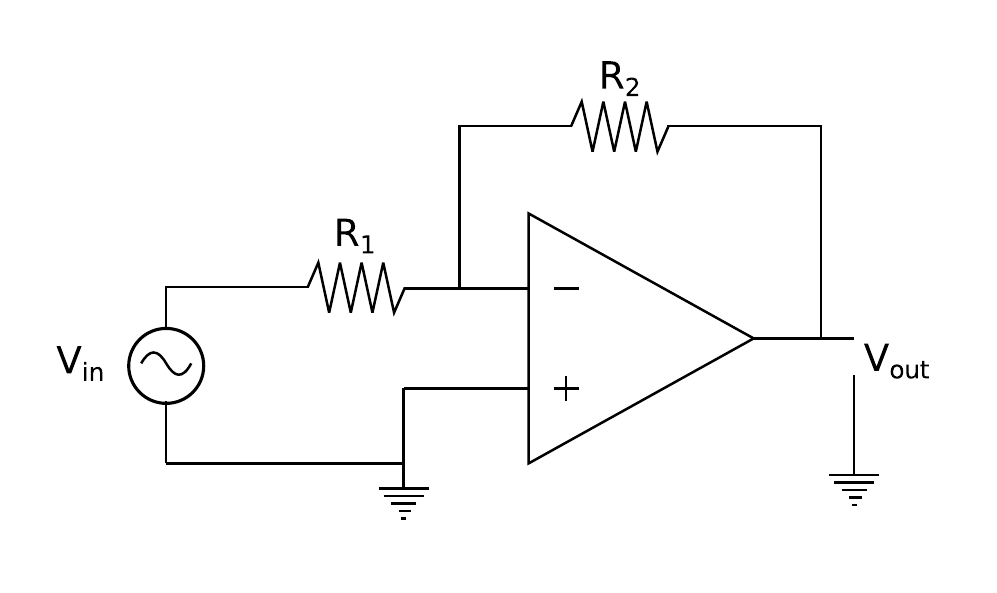
\includegraphics[width=0.5\linewidth]{imgs/intro_1.png}
	\caption{Basic configuration}
	\label{fig-intro-1}
\end{figure}

The relationship that you’re going to analyze is the amplification of a $V_{in}=0.1$ V and the
output should be: 1, 5, 10 and 20 V. For a separated experiment, change the source
for a sinusoidal one with $V_{in}=0.2$ V and output 10 V, with a frequency variation for 100
Hz, 500 Hz, 5 kHz, 100 kHz, 2 MHz, 10 MHz and 20 MHz.


\subsection{Filters}
For the second circuit, a filter or filters are in order to be analyzed, as shown in Figure \ref{fig-intro-2-1} \& \ref{fig-intro-2-2} simulate and fabricated. Figure shows the diagram of the filter that is required
to be analyzed.

\begin{figure}[htbp]
	\centering
	\subfigure[High-pass filter]{
		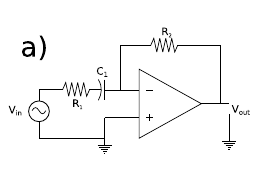
\includegraphics[width=0.45\linewidth]{imgs/intro_2.png}
		\label{fig-intro-2-1}
	}
	\subfigure[Low-pass filter]{
		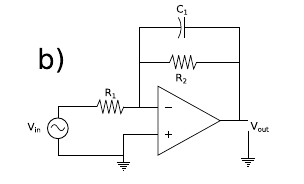
\includegraphics[width=0.45\linewidth]{imgs/intro_3.png}
		\label{fig-intro-2-2}
	}
	\caption{Basic configuration for active filters.}
	\label{fig-intro-2}
\end{figure}

Calculate the right values for capacitors and resistors in order to get the follow cut-off frequencies: 2 kHz, 10 kHz and 1 MHz.

\newpage

\section{Experimental results and discussion}

\subsection{Simple amplifier}

In order to get output of 1, 5, 10 and 20 V, we use $R_1=1\unit{k\Omega}$ and $R_2=$ 1, 5, 10 and 20 $\rm{k\Omega}$. The result was shown in Figure \ref{fig-1-1}.

\begin{figure}[htbp]
	\centering
	\subfigure[gain=1]{
		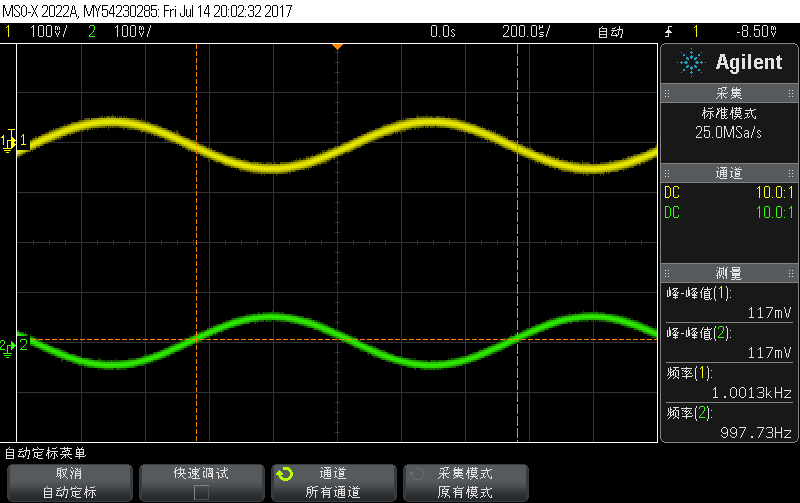
\includegraphics[width=0.45\linewidth]{imgs/scope_23.png}
		\label{fig-1-1-1}
	}
	\subfigure[gain=5]{
		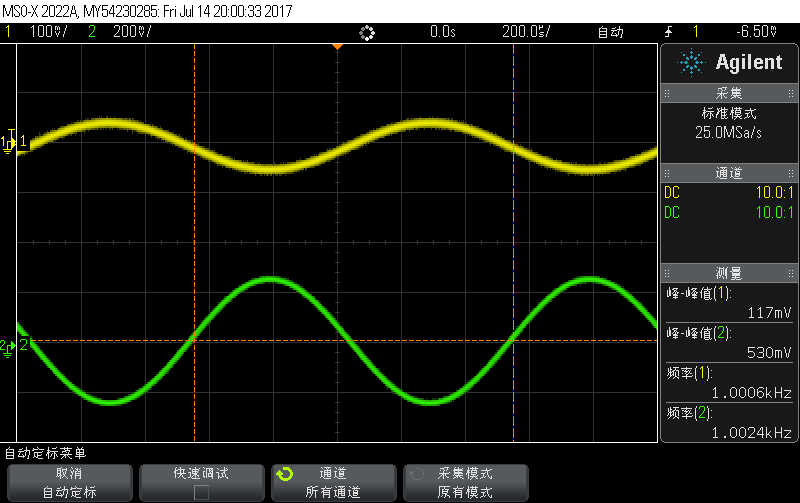
\includegraphics[width=0.45\linewidth]{imgs/scope_20.png}
		\label{fig-1-1-2}
	}
	\subfigure[gain=10]{
		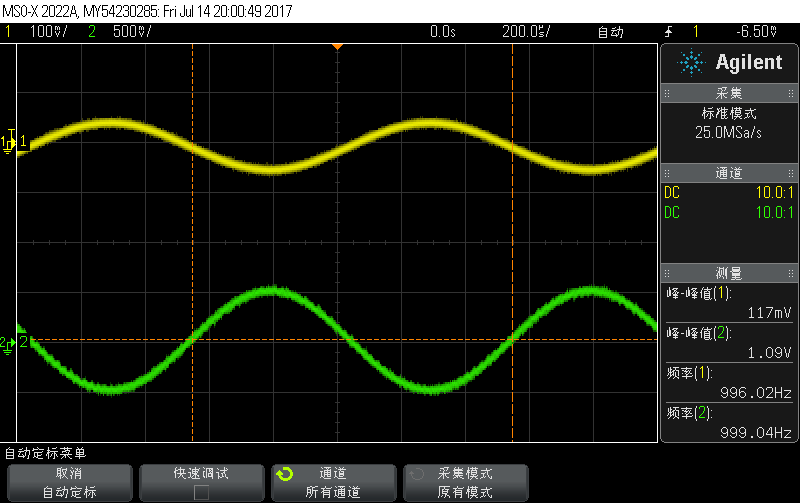
\includegraphics[width=0.45\linewidth]{imgs/scope_21.png}
		\label{fig-1-1-3}
	}
	\subfigure[gain=20]{
		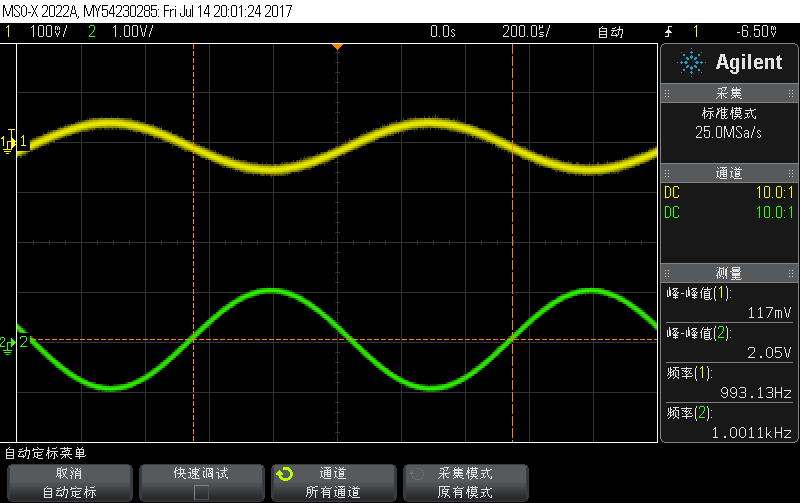
\includegraphics[width=0.45\linewidth]{imgs/scope_22.png}
		\label{fig-1-1-4}
	}
	\caption{Analysis of amplification with different gain.}
	\label{fig-1-1}
\end{figure}


Change the source for a sinusoidal one with $V_{in}=0.2$ V and output 10 V, with a frequency variation for 100 Hz, 500 Hz, 5 kHz, 100 kHz, 2 MHz, 10 MHz and 20 MHz. The result was shown in Figure \ref{fig-1-2}.

\begin{figure}[htbp]
	\centering
	\subfigure[100 Hz]{
		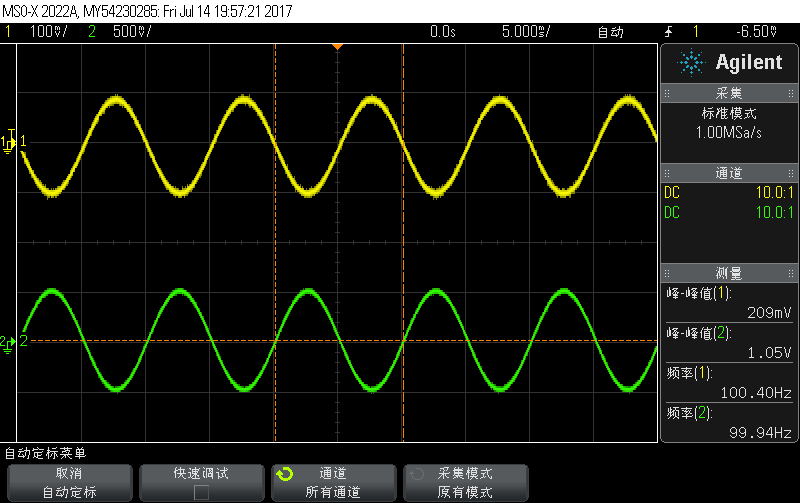
\includegraphics[width=0.45\linewidth]{imgs/scope_13.png}
		\label{fig-1-2-1}
	}
	\subfigure[500 Hz]{
		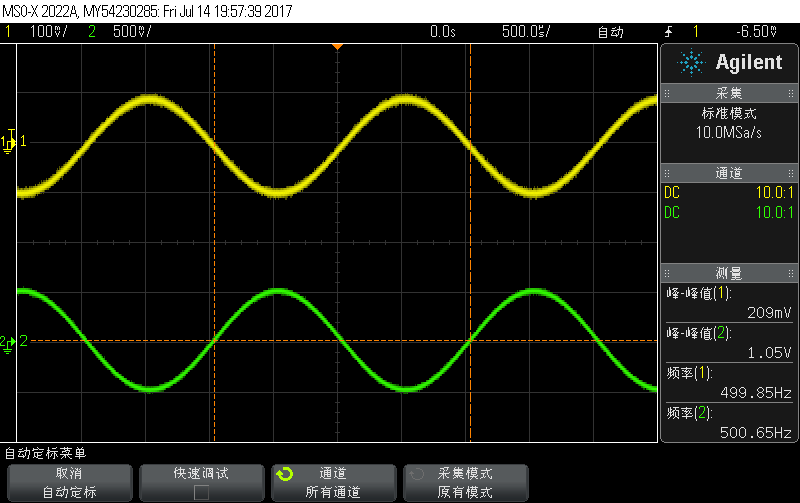
\includegraphics[width=0.45\linewidth]{imgs/scope_14.png}
		\label{fig-1-2-2}
	}
	\subfigure[5 kHz]{
		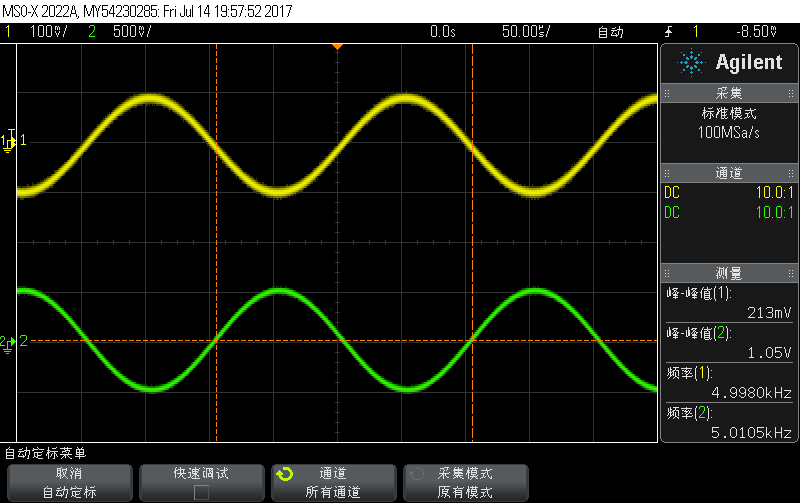
\includegraphics[width=0.45\linewidth]{imgs/scope_15.png}
		\label{fig-1-2-3}
	}
	\subfigure[100 kHz]{
		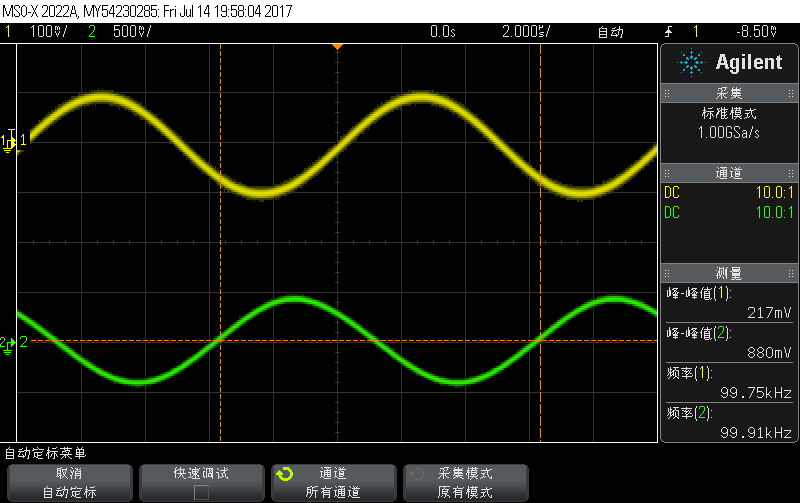
\includegraphics[width=0.45\linewidth]{imgs/scope_16.png}
		\label{fig-1-2-4}
	}
	\subfigure[2 MHz]{
		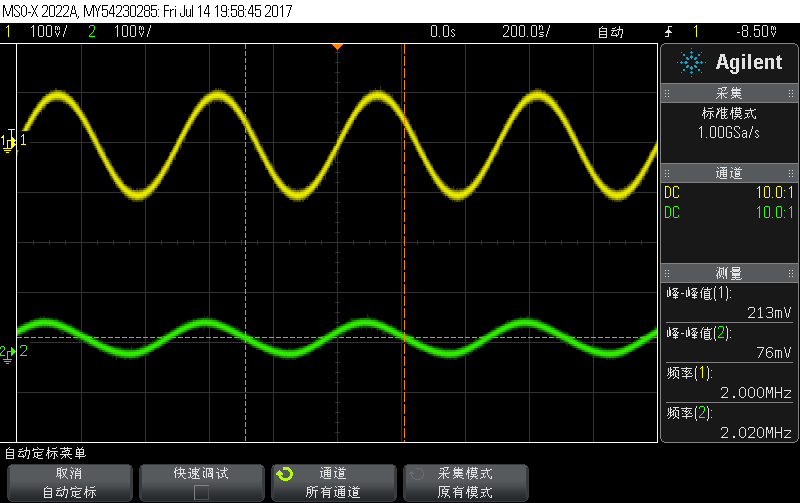
\includegraphics[width=0.45\linewidth]{imgs/scope_17.png}
		\label{fig-1-2-5}
	}
	\subfigure[10 MHz]{
		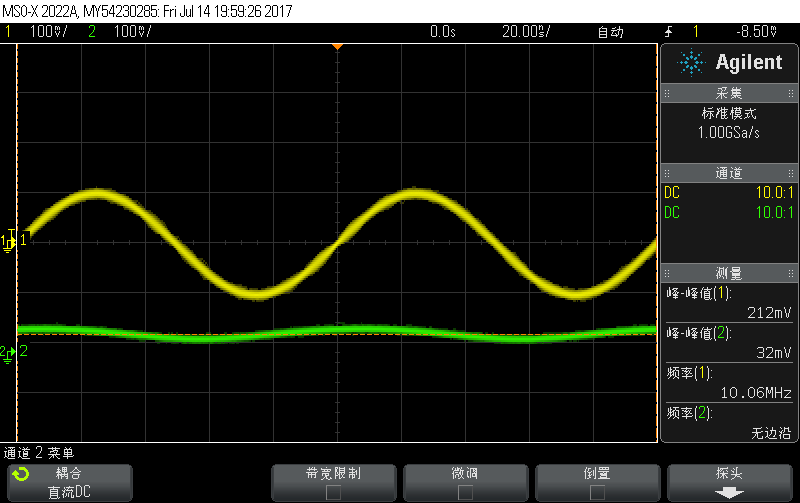
\includegraphics[width=0.45\linewidth]{imgs/scope_18.png}
		\label{fig-1-2-6}
	}
	\subfigure[20 MHz]{
		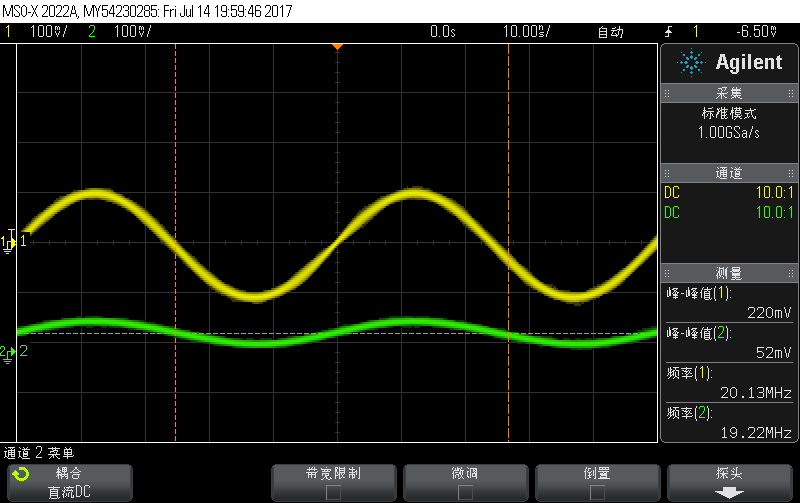
\includegraphics[width=0.45\linewidth]{imgs/scope_19.png}
		\label{fig-1-2-7}
	}
	\caption{Analysis of amplification with different frequency.}
	\label{fig-1-2}
\end{figure}

The simulation result was shown in \ref{fig-1-3}.

\begin{figure}[htbp]
	\centering
	\subfigure[100 Hz]{
		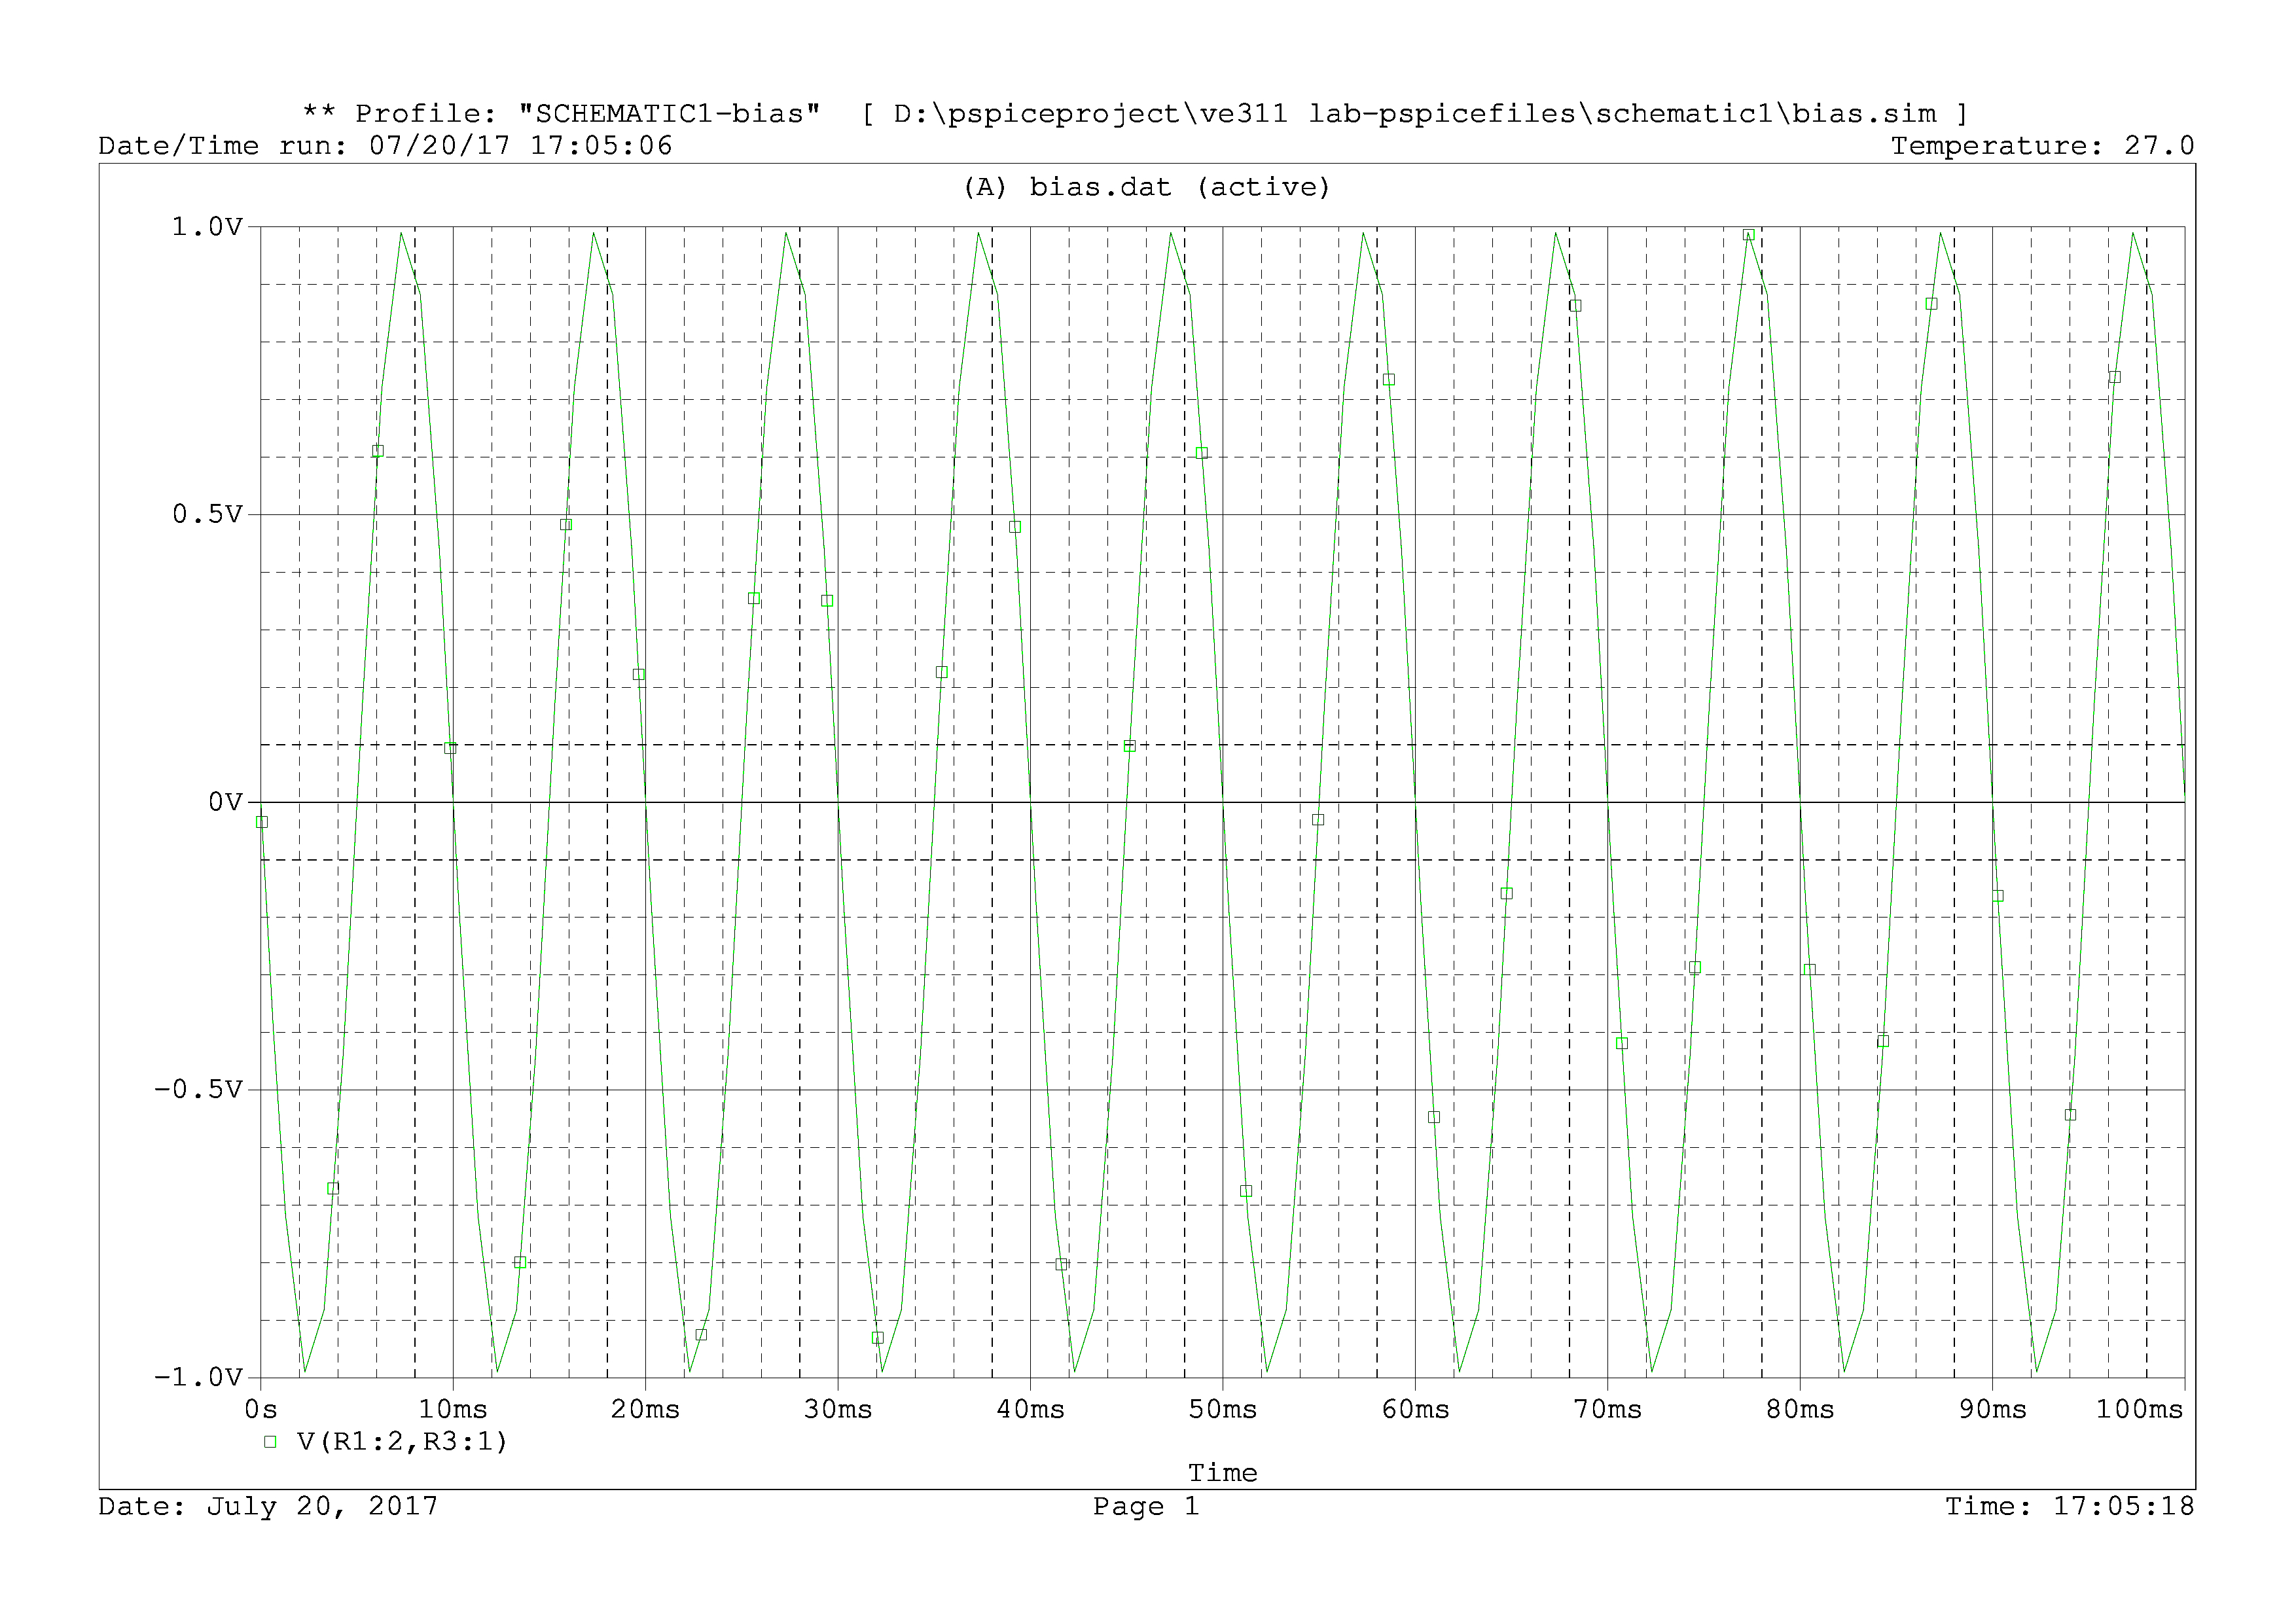
\includegraphics[width=0.4\linewidth]{imgs/100.png}
		\label{fig-1-3-1}
	}
	\subfigure[500 Hz]{
		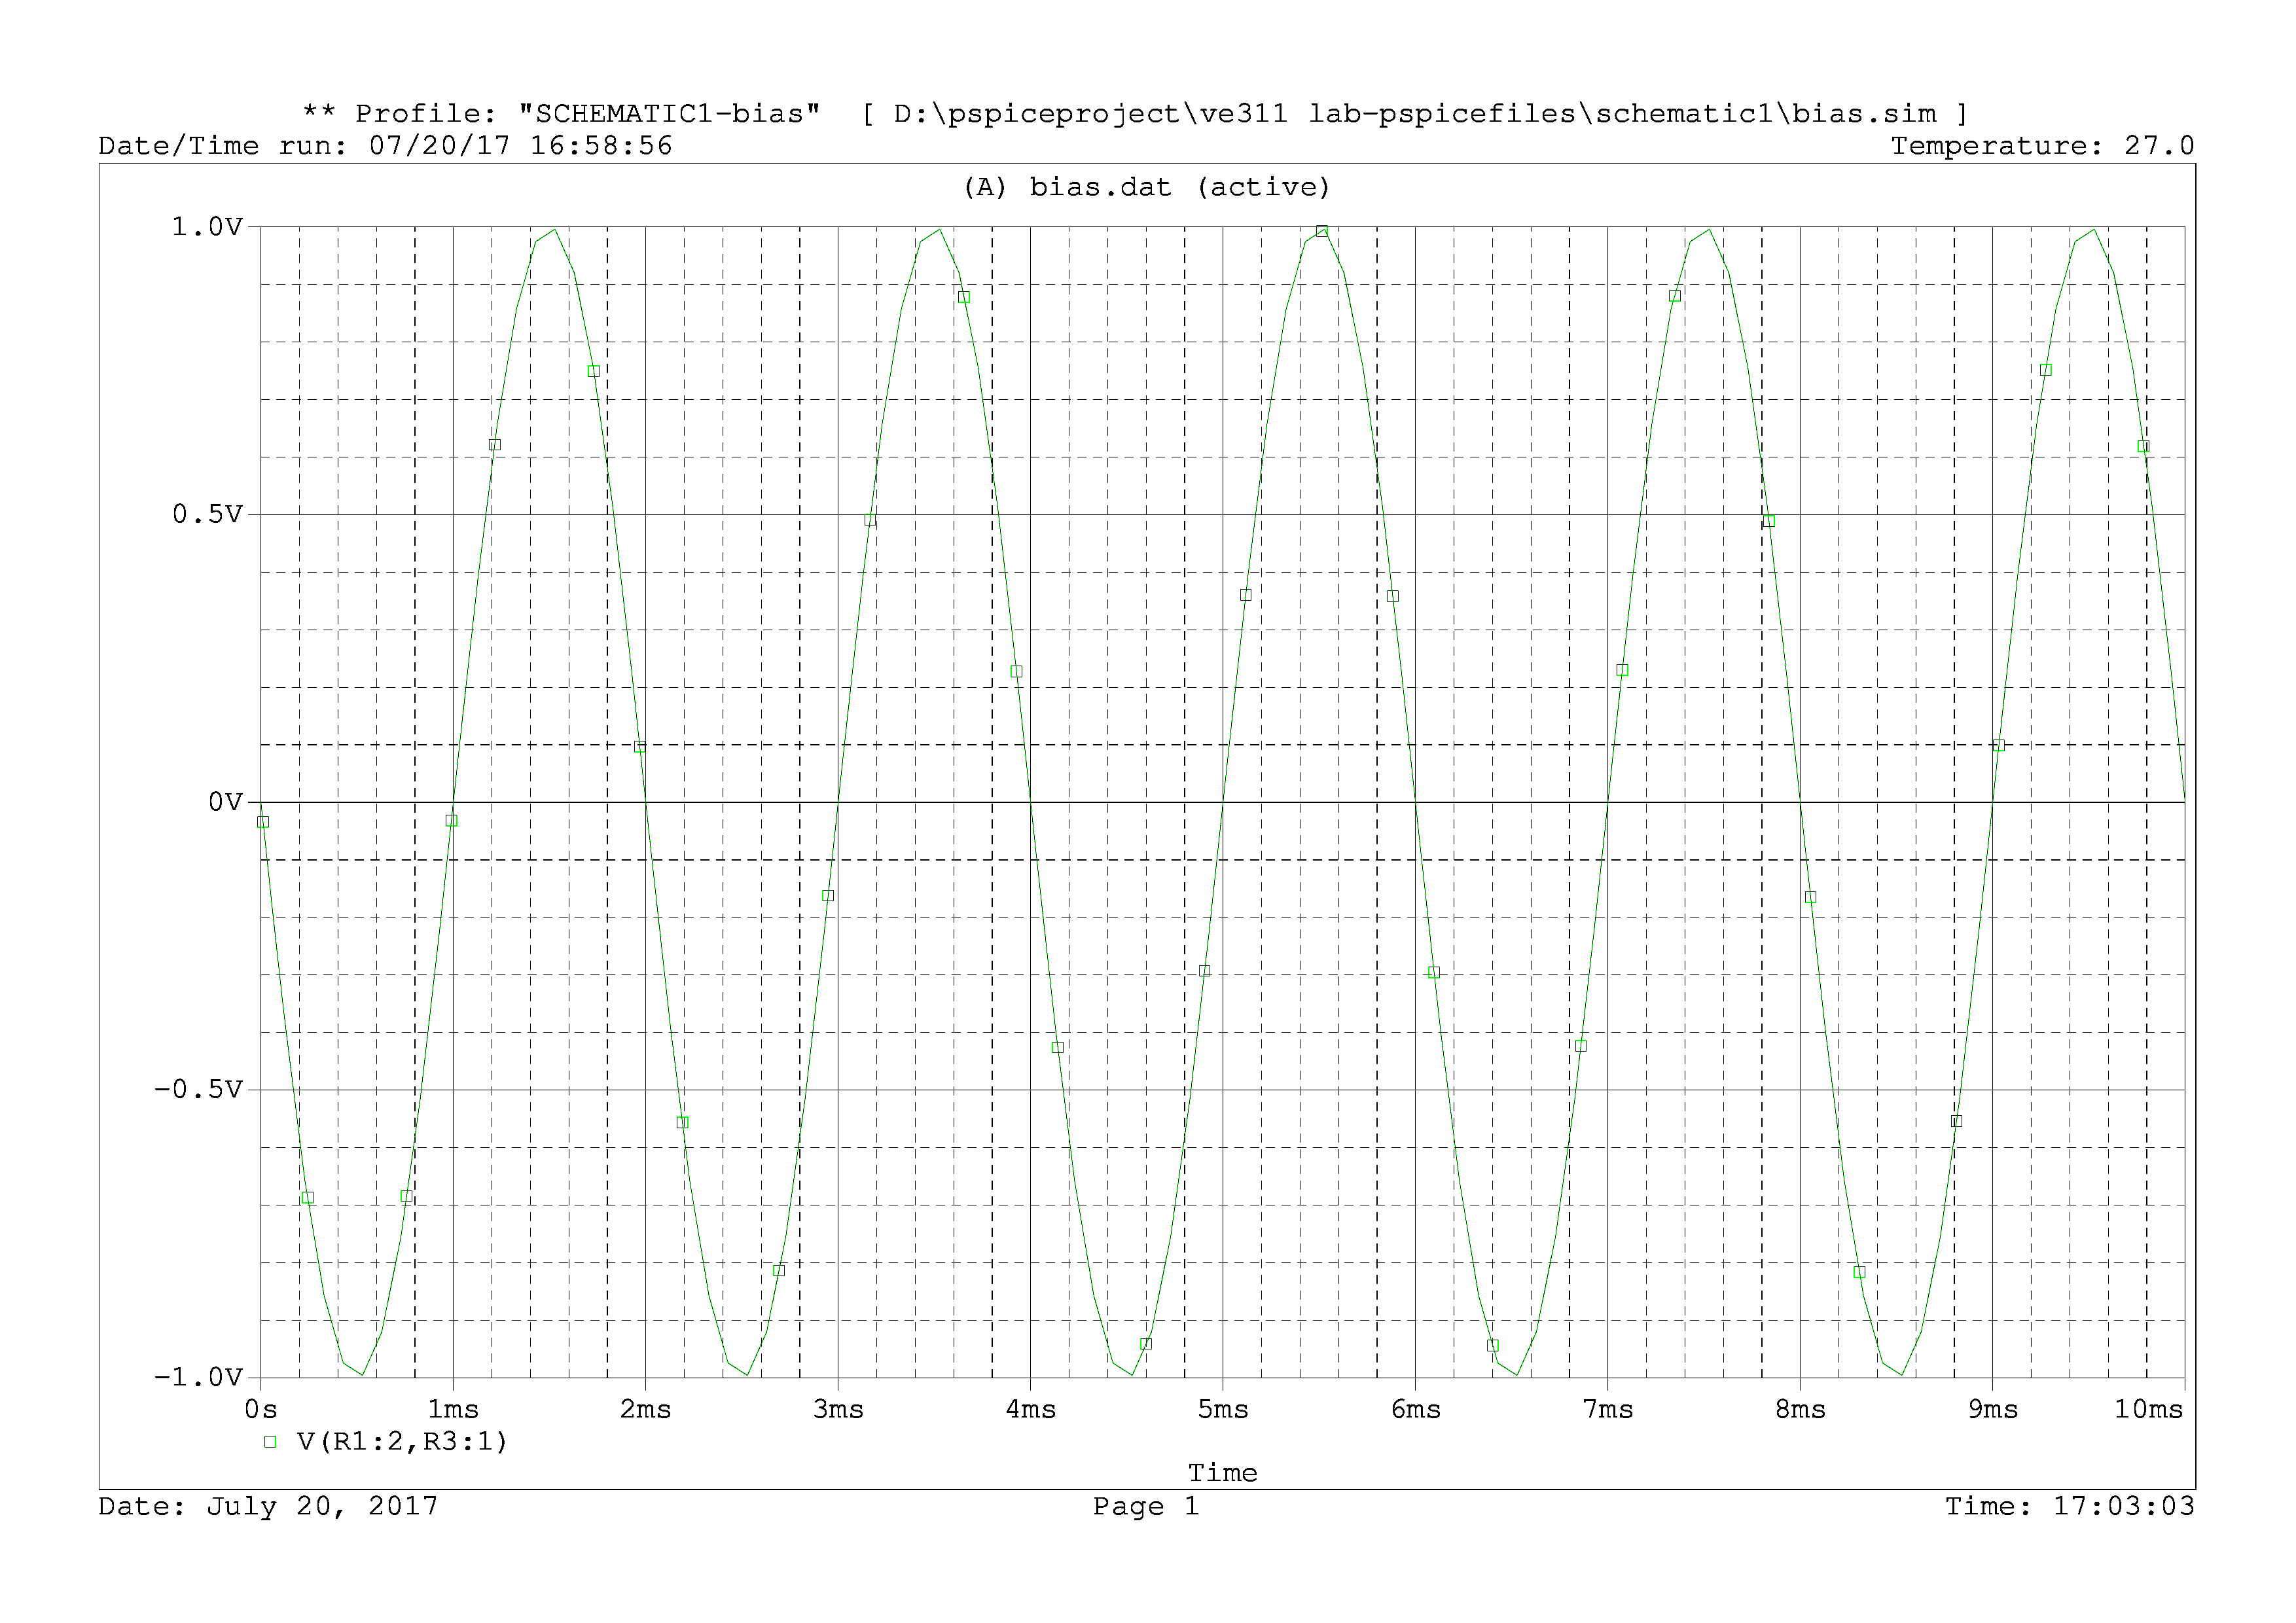
\includegraphics[width=0.4\linewidth]{imgs/500.png}
		\label{fig-1-3-2}
	}
	\subfigure[5 kHz]{
		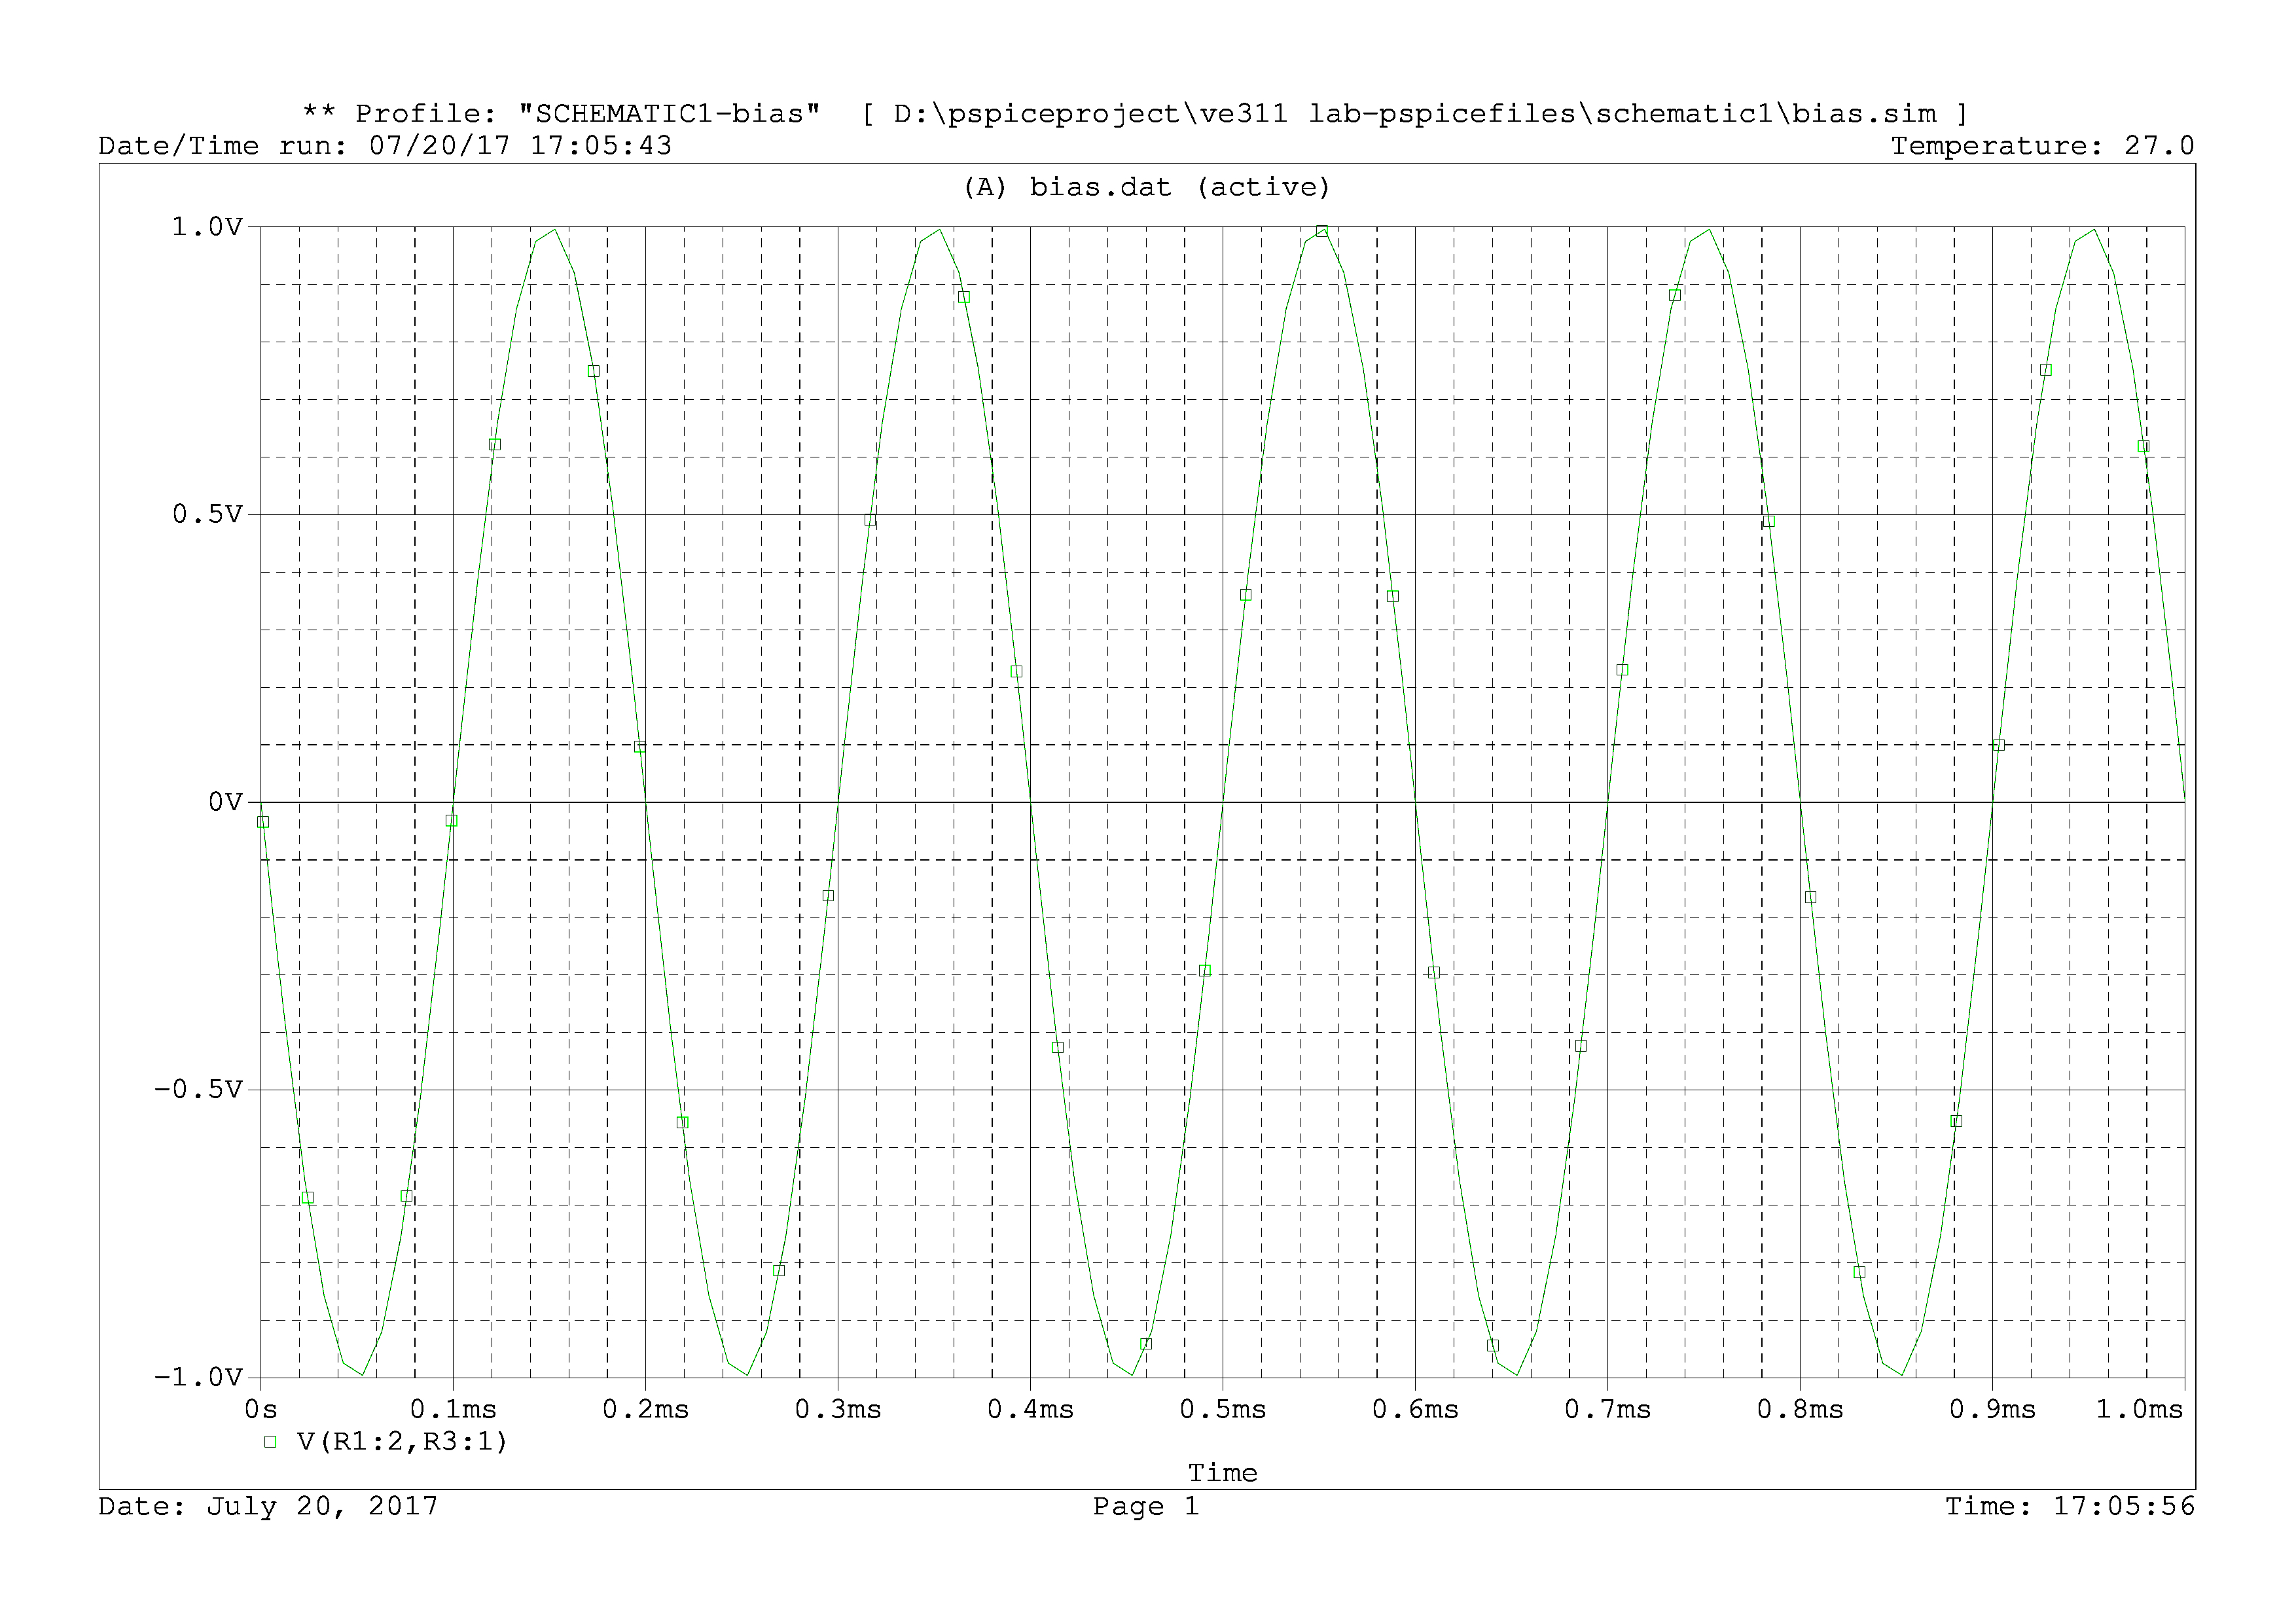
\includegraphics[width=0.4\linewidth]{imgs/5k.png}
		\label{fig-1-3-3}
	}
	\subfigure[100 kHz]{
		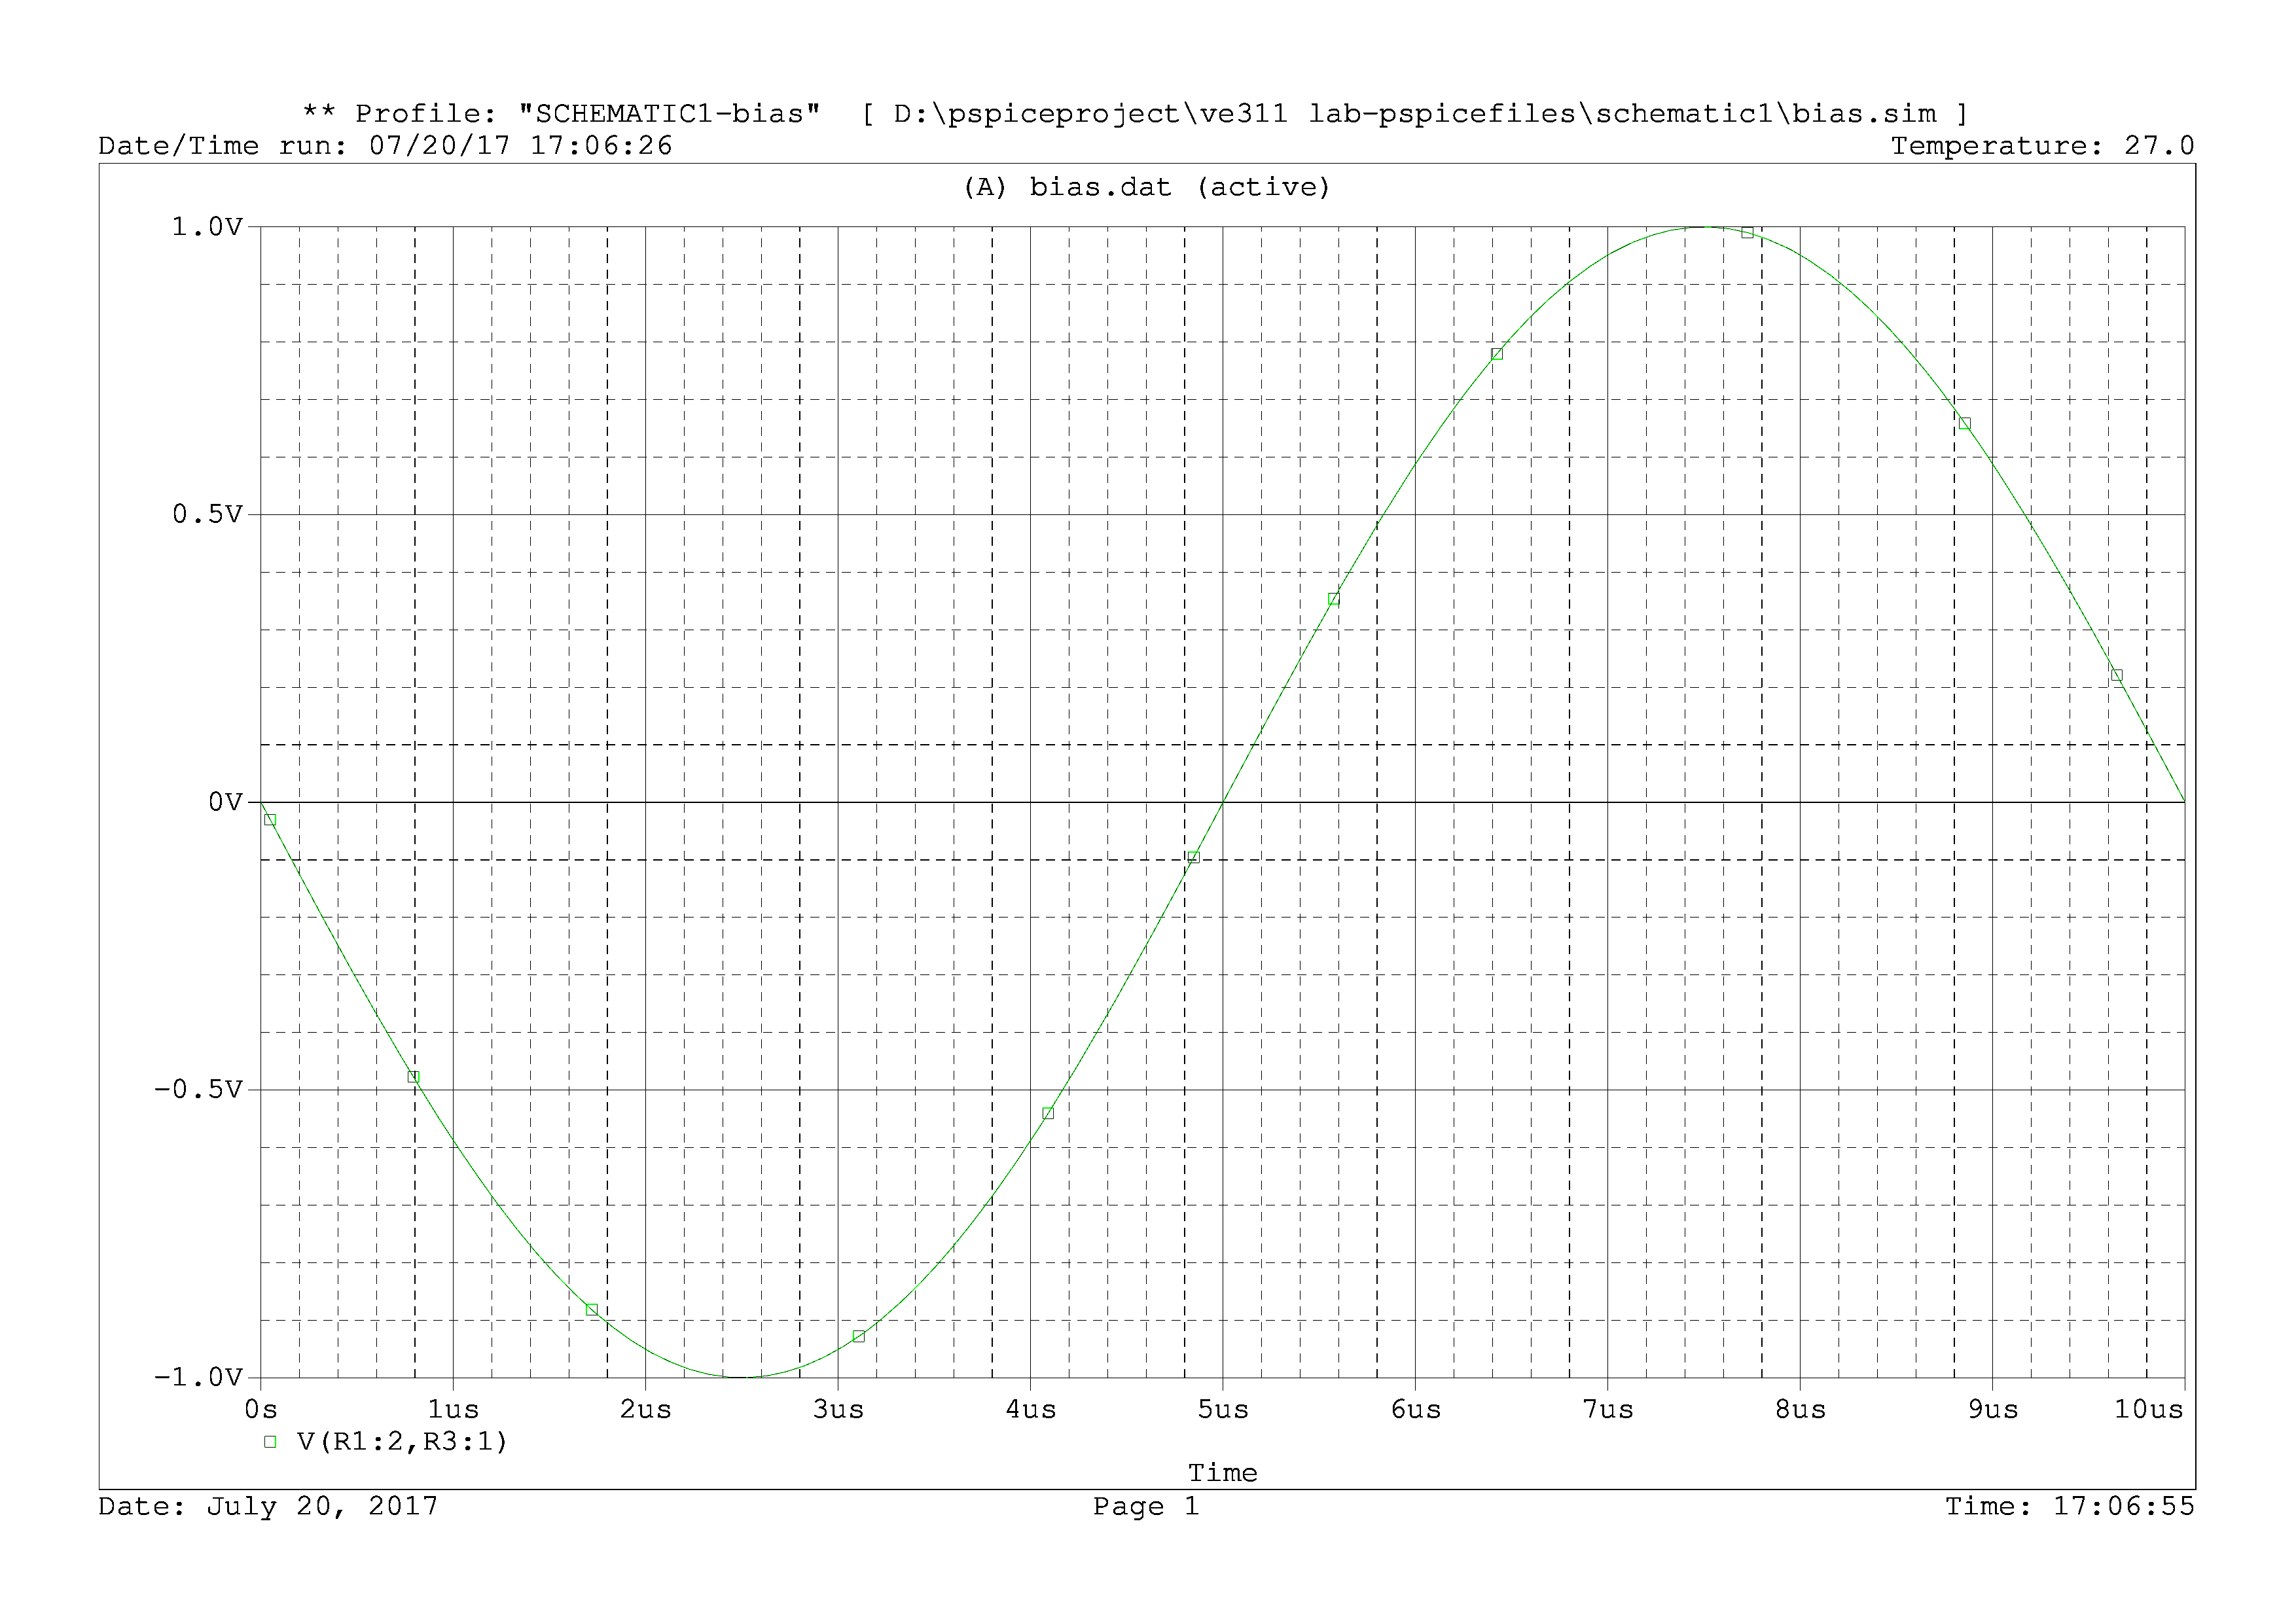
\includegraphics[width=0.4\linewidth]{imgs/100k.png}
		\label{fig-1-3-4}
	}
	\subfigure[2 MHz]{
		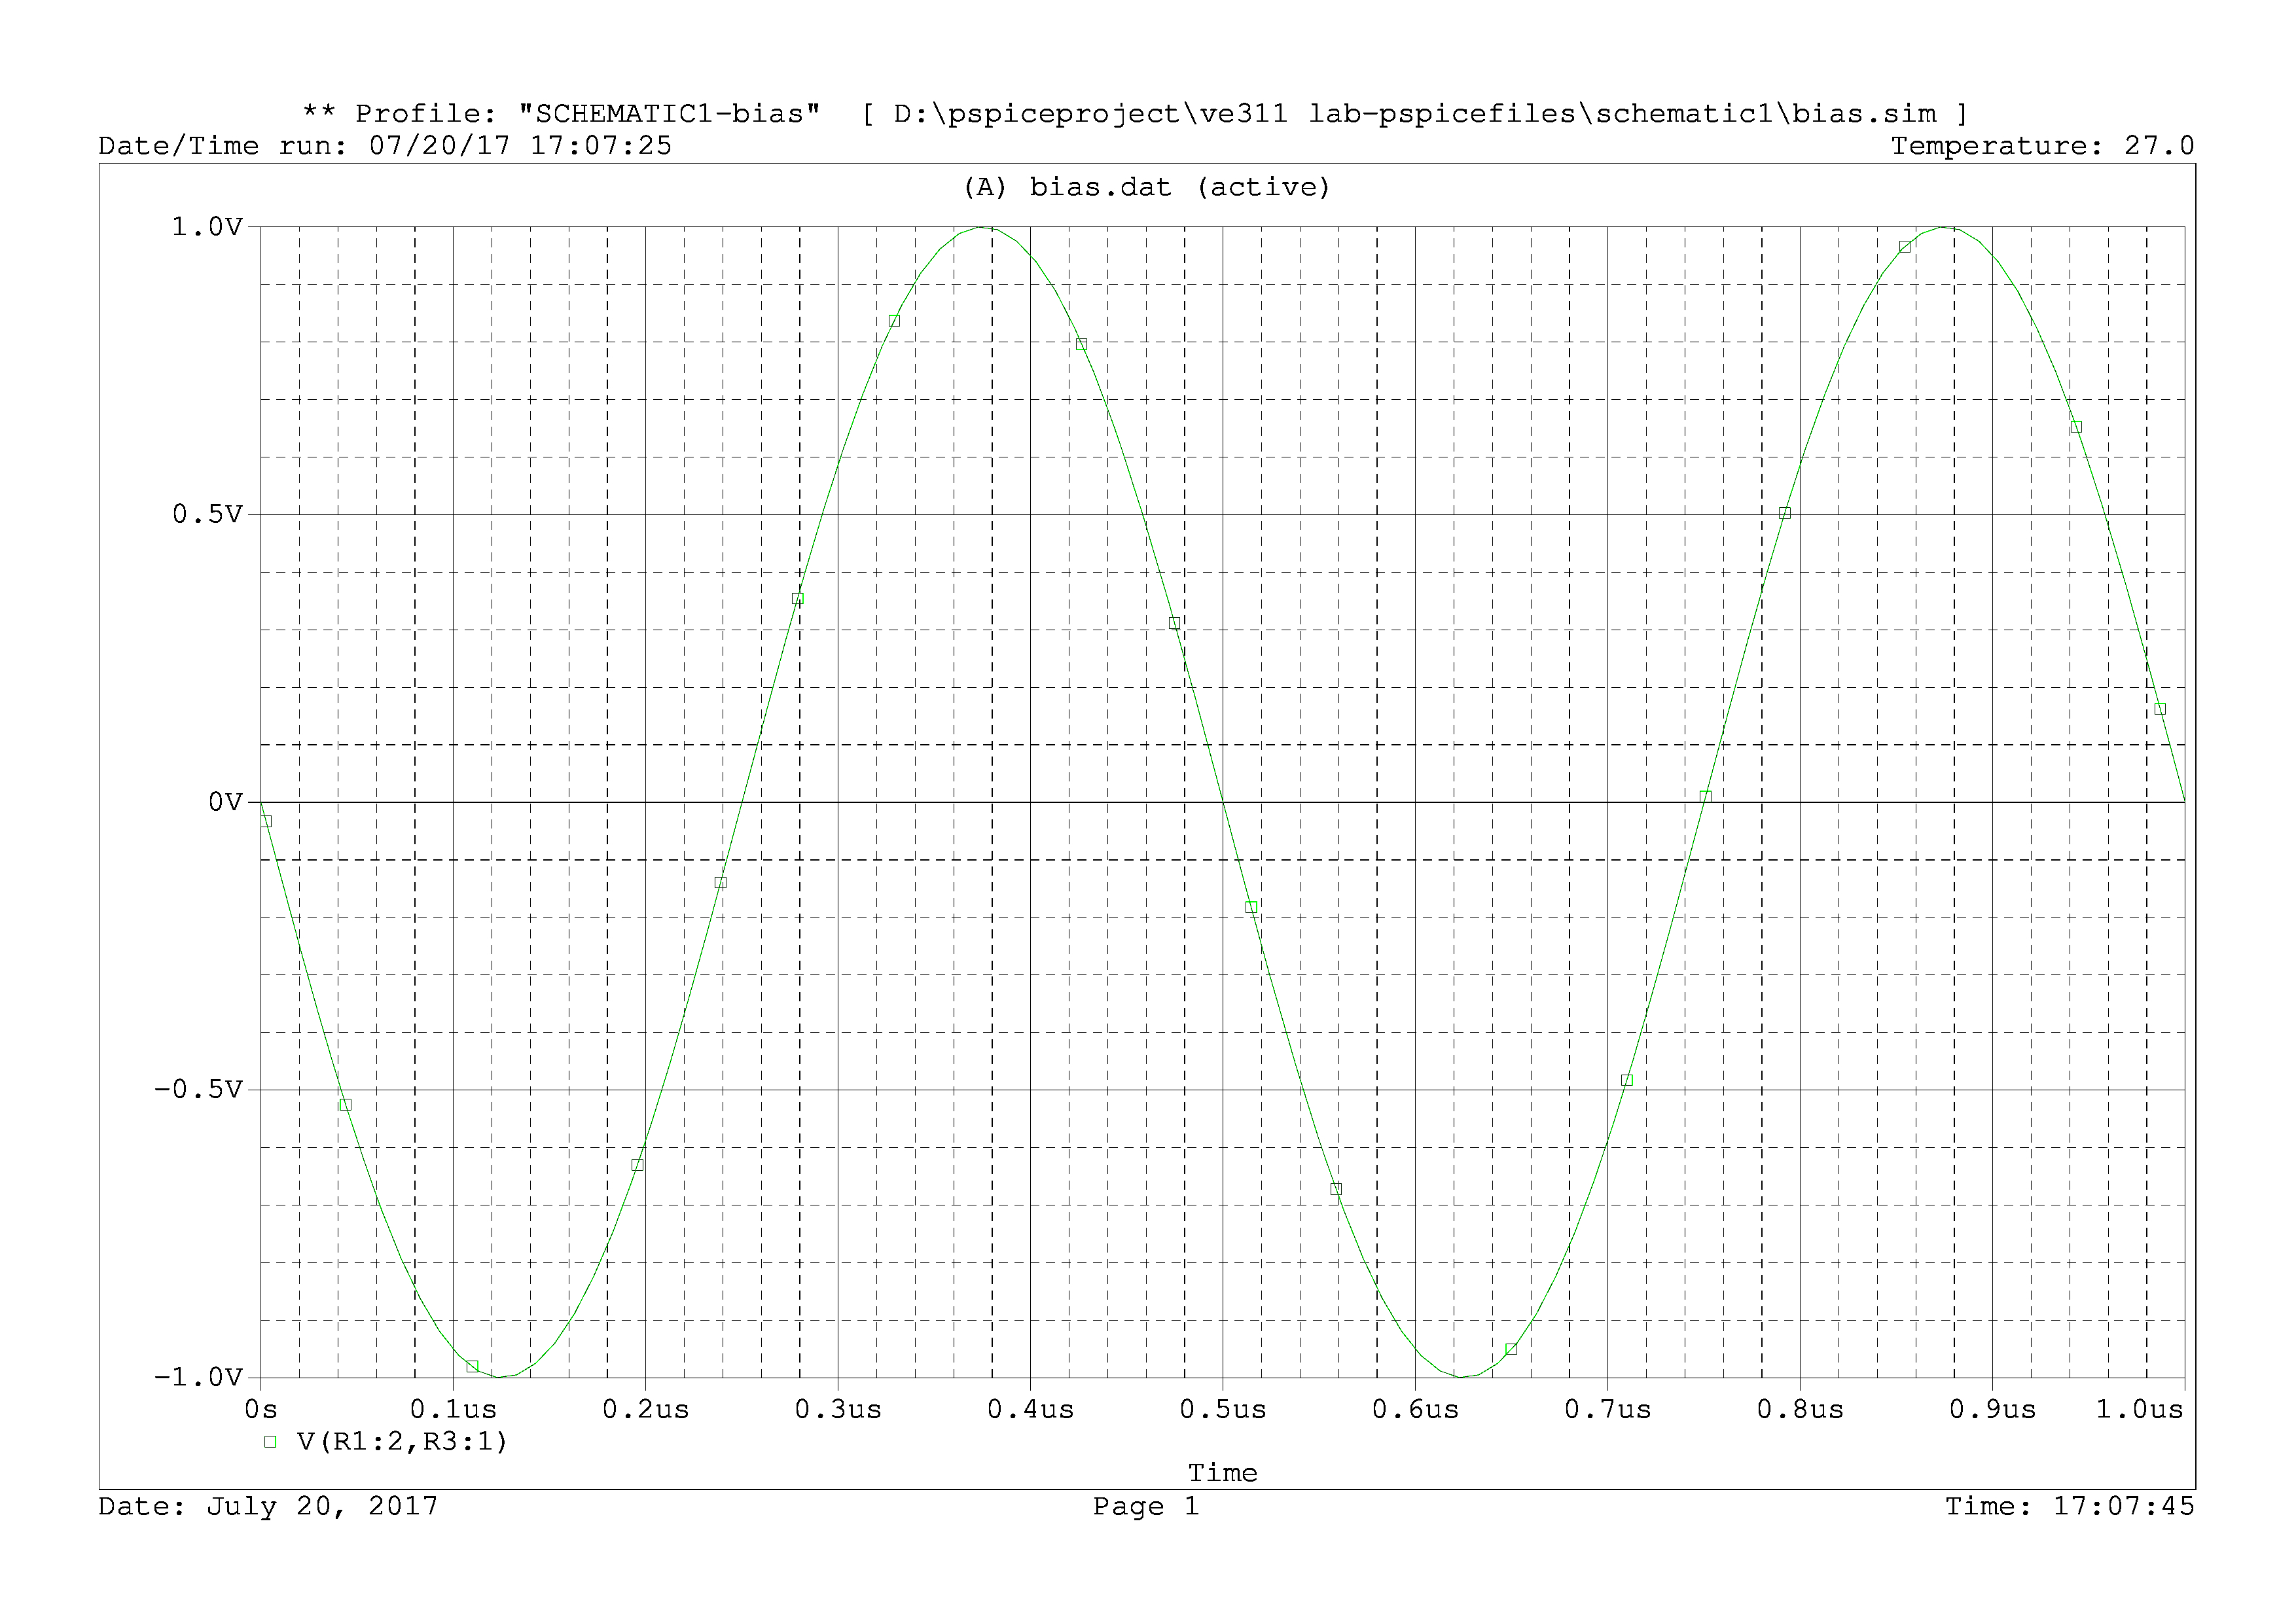
\includegraphics[width=0.4\linewidth]{imgs/2M.png}
		\label{fig-1-3-5}
	}
	\subfigure[10 MHz]{
		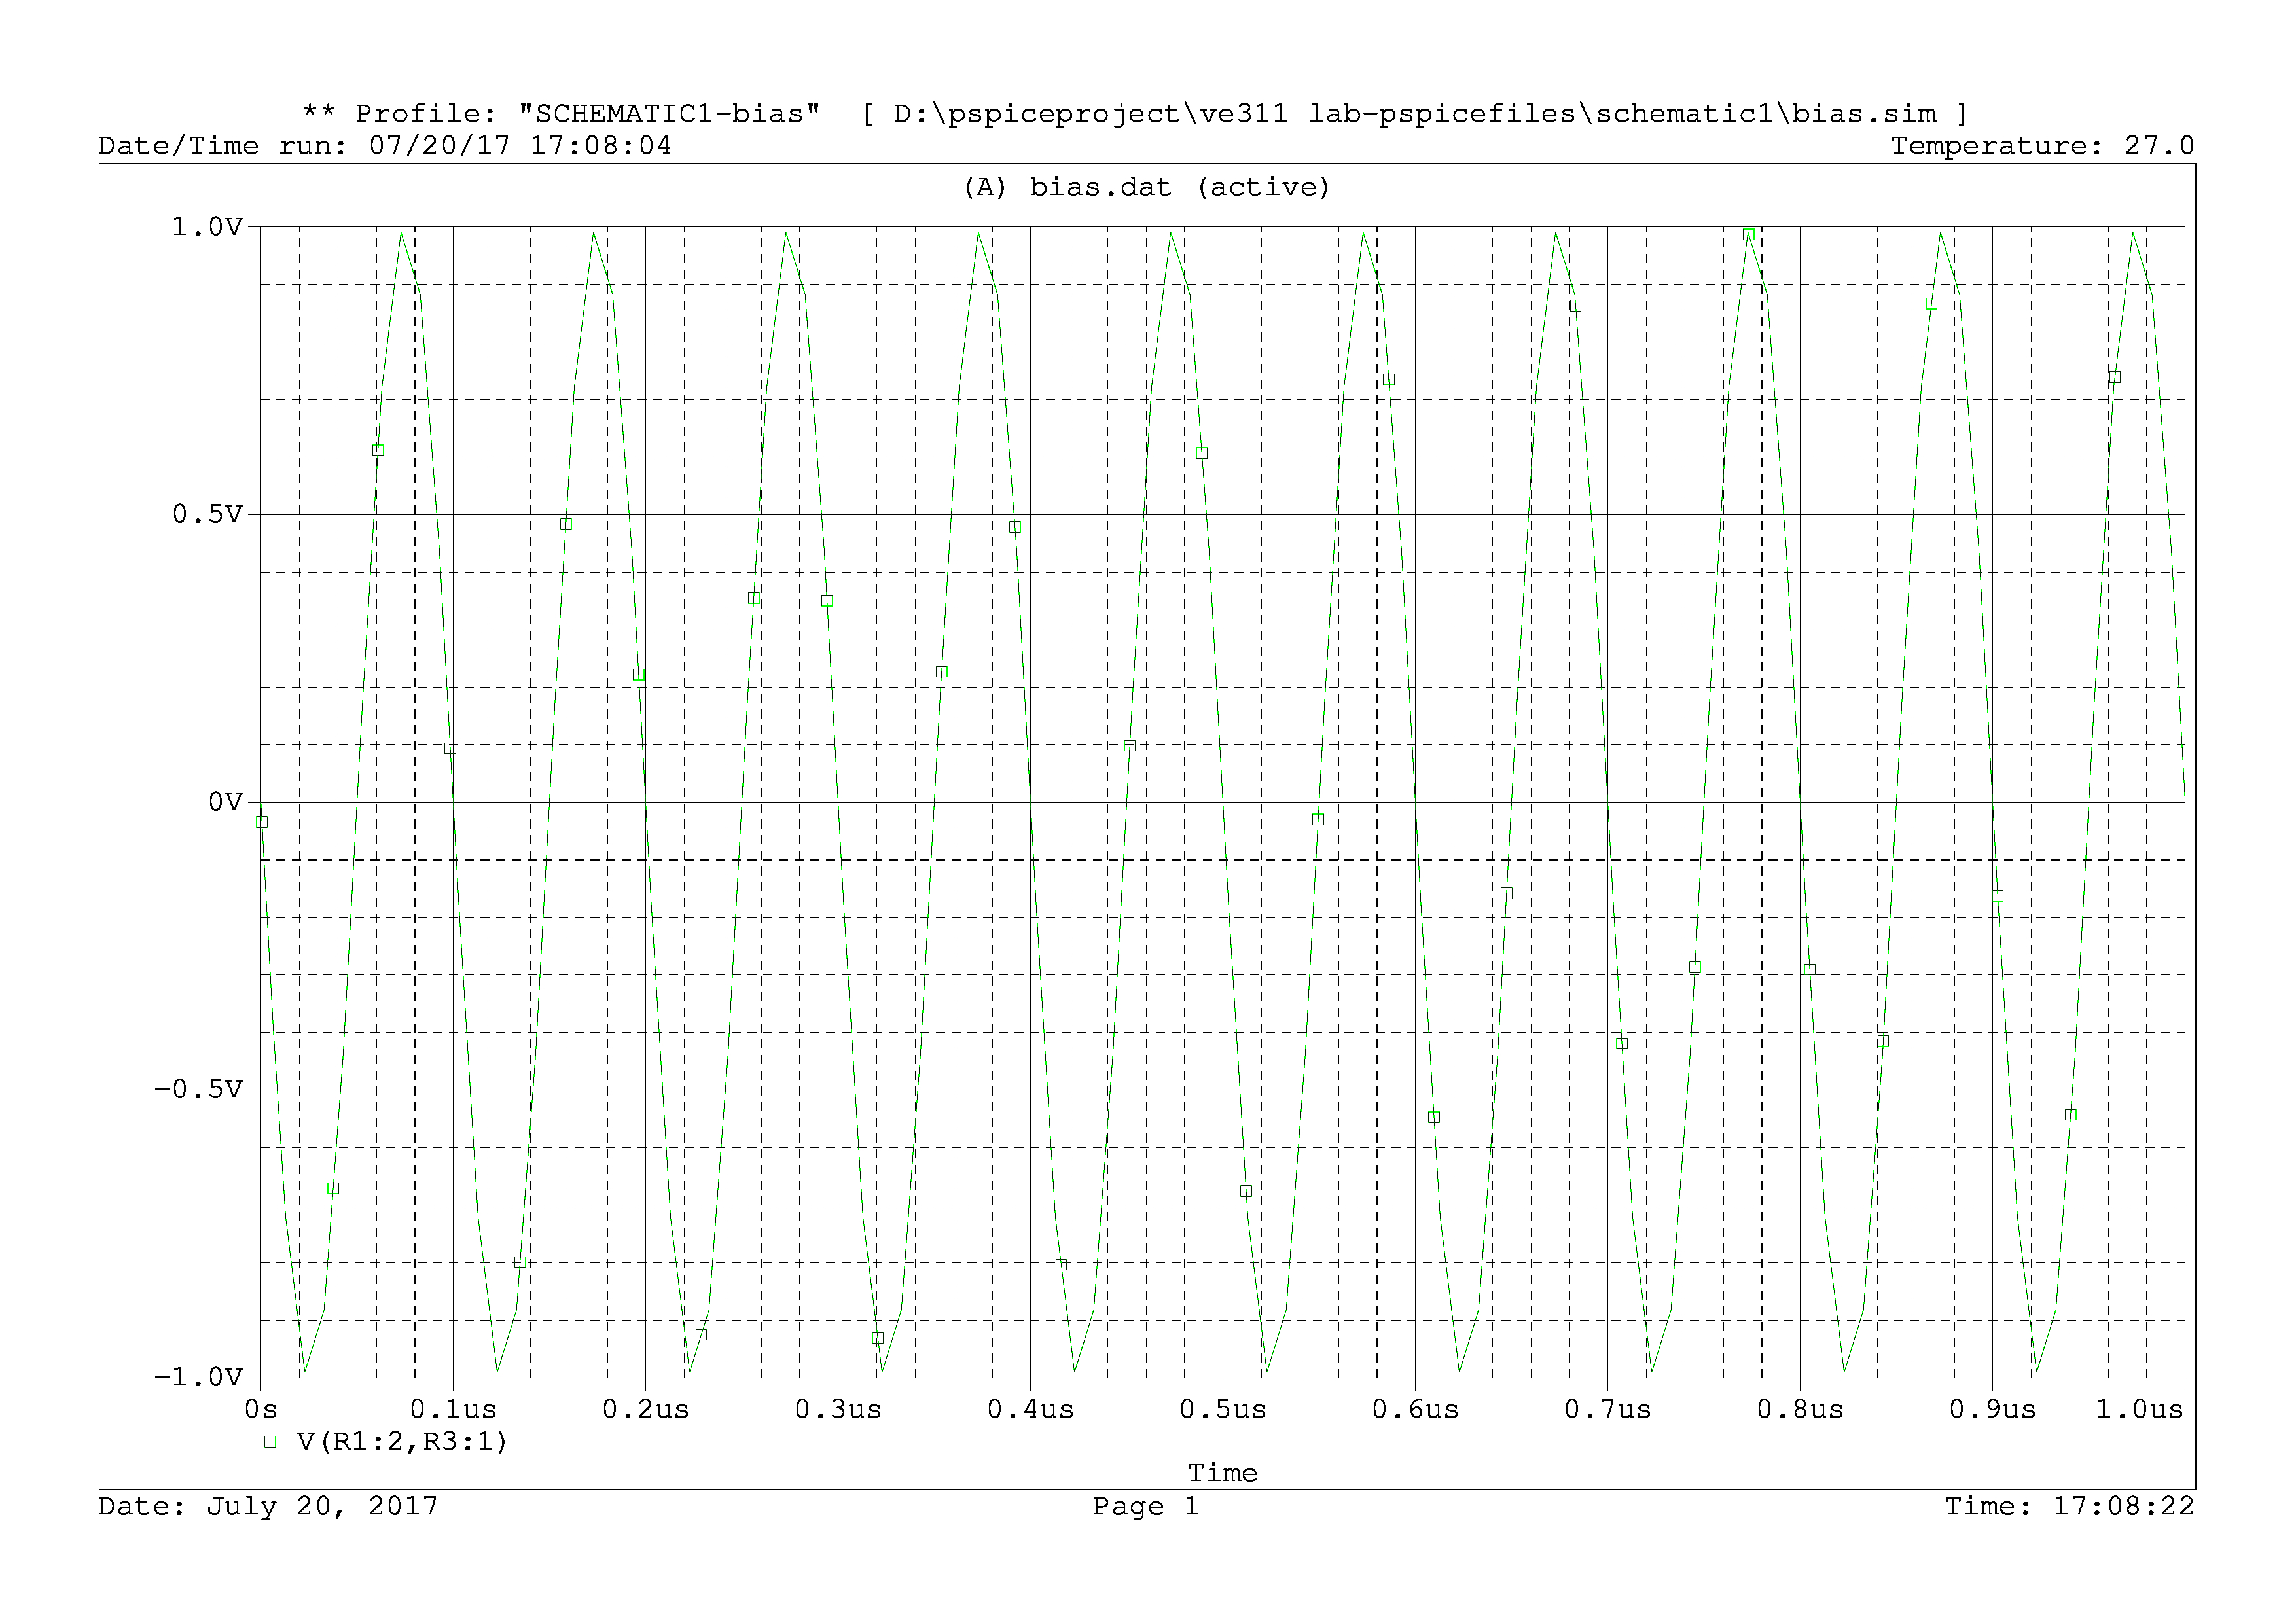
\includegraphics[width=0.4\linewidth]{imgs/10M.png}
		\label{fig-1-3-6}
	}
	\subfigure[20 MHz]{
		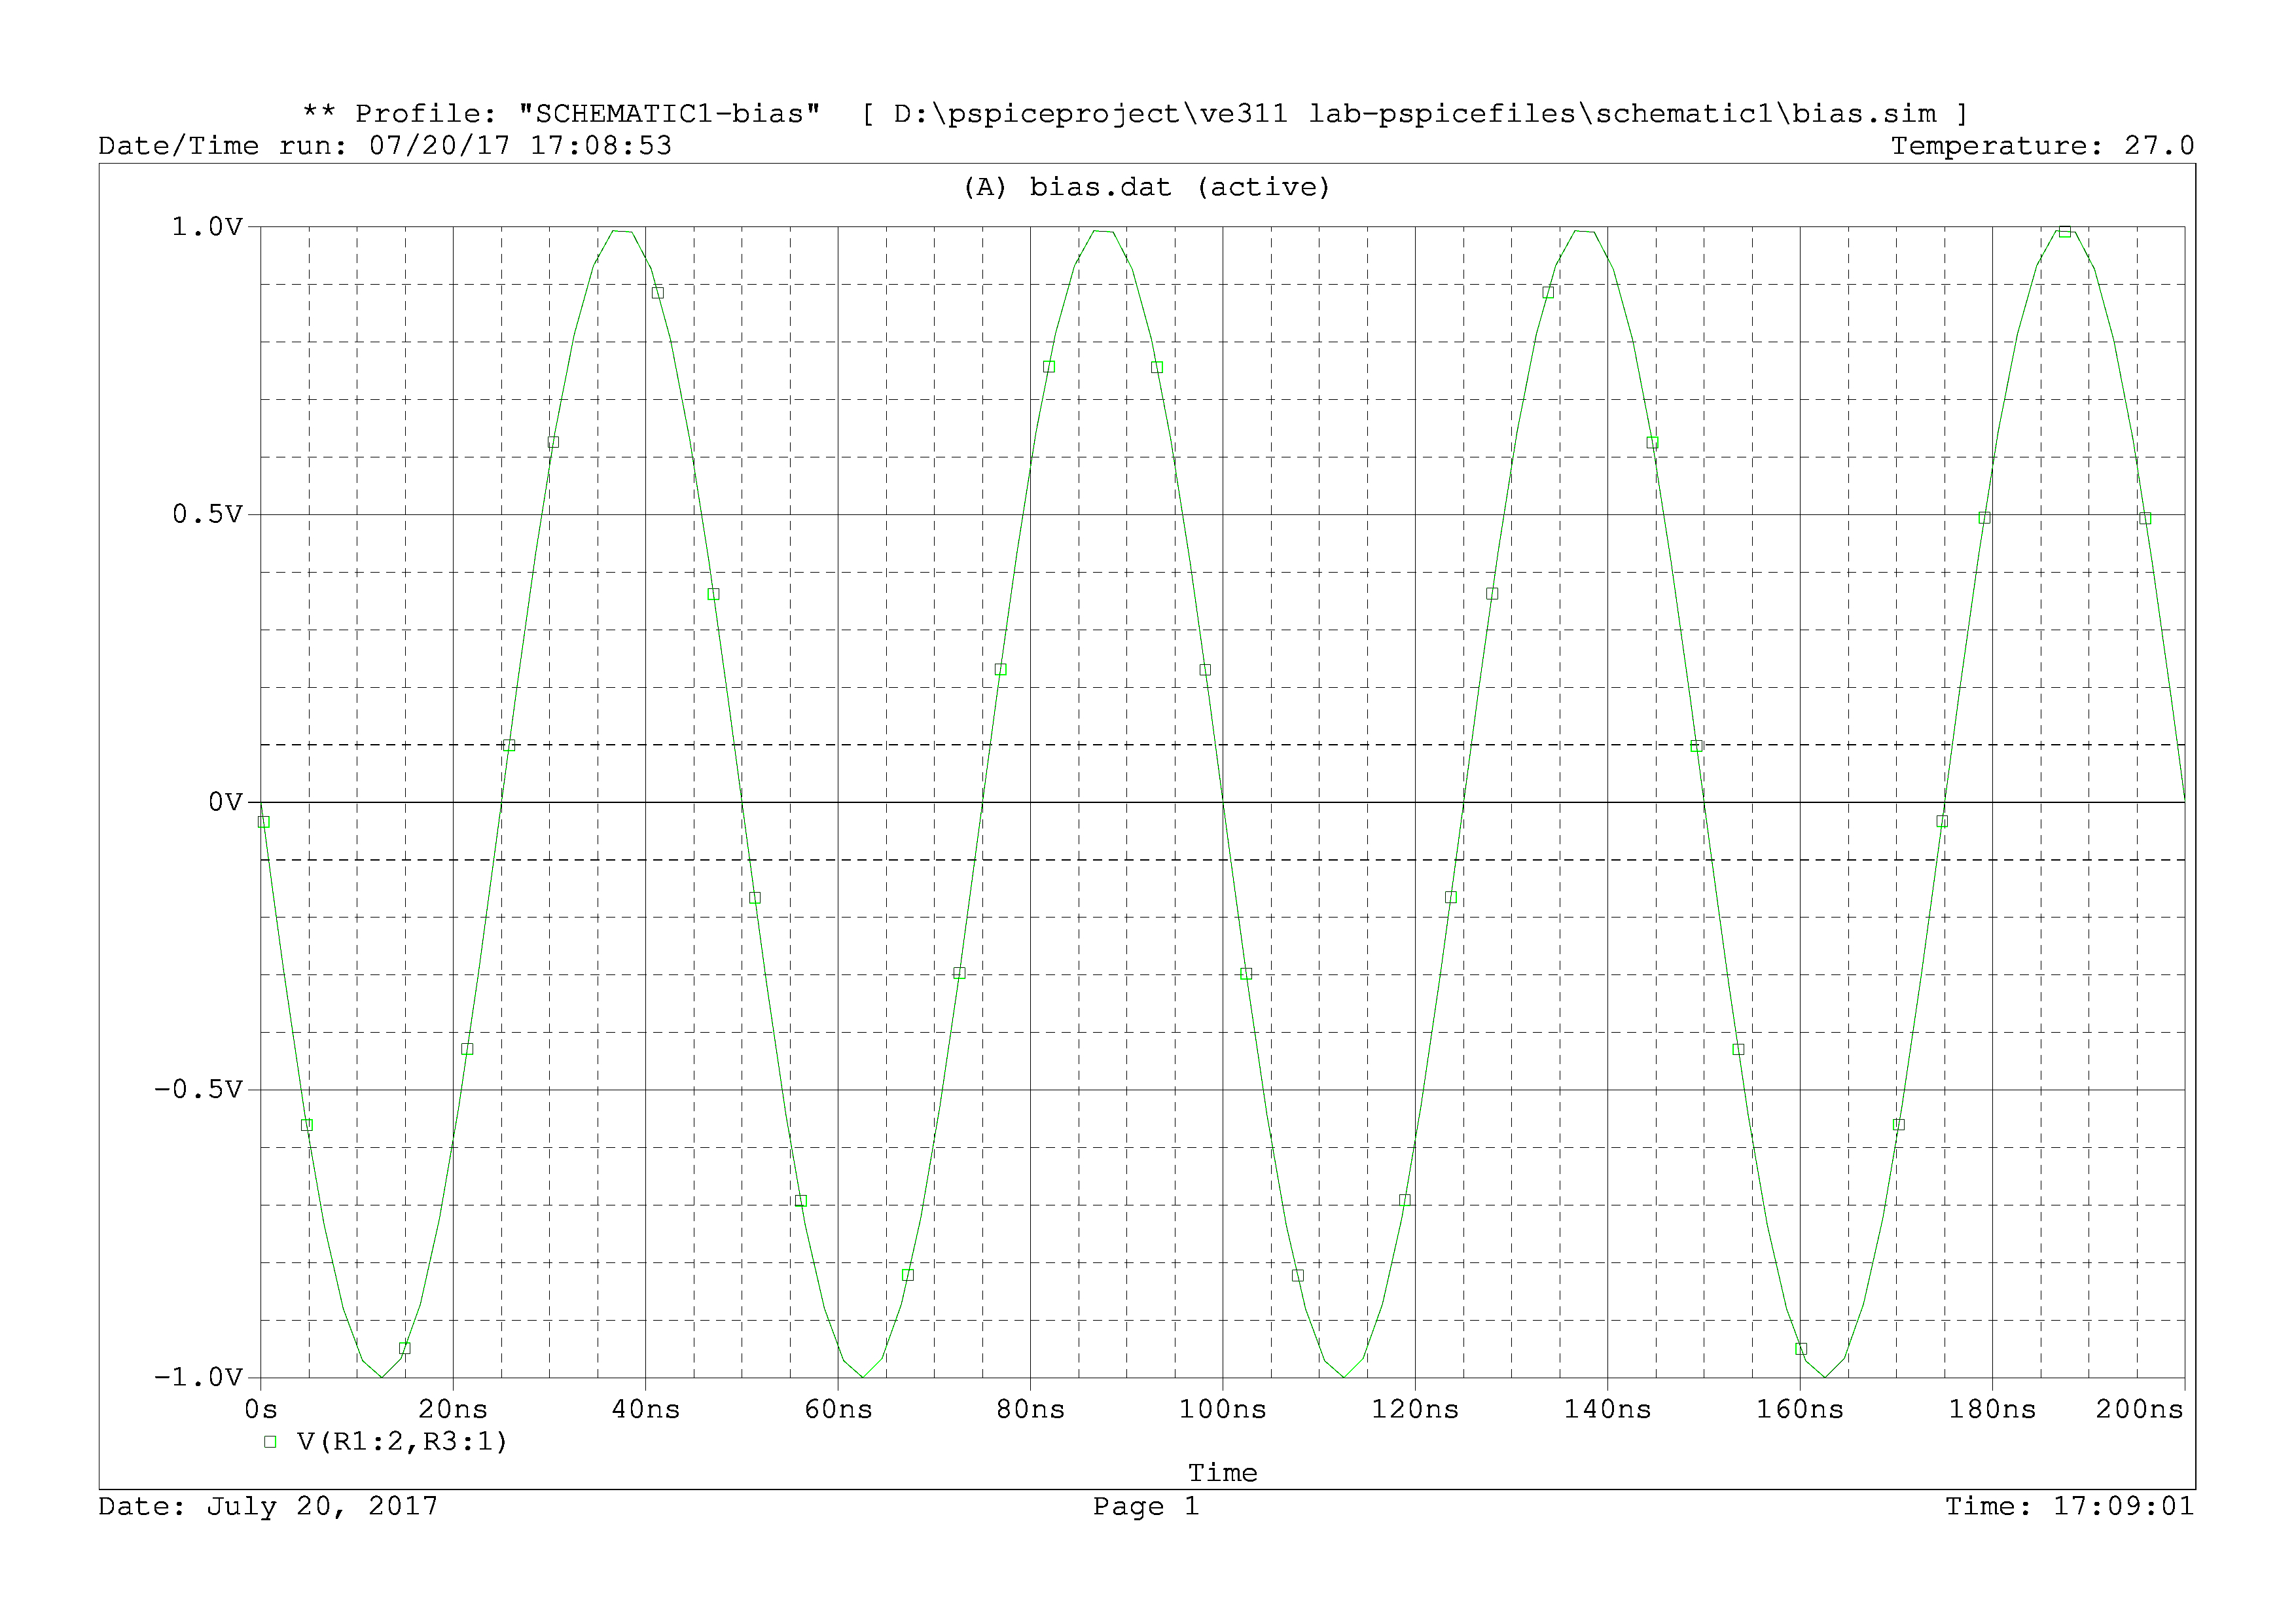
\includegraphics[width=0.4\linewidth]{imgs/20M.png}
		\label{fig-1-3-7}
	}
	\caption{Simulation of amplification with different frequency.}
	\label{fig-1-3}
\end{figure}

\newpage

\subsection{Filters}

When cut-off frequency is 2 kHz, and $R_1=1\unit{k\Omega}$, $R_2=5\unit{k\Omega}$, we can calculate the value of $C$.

\subsubsection{High-pass filter}

$$f=\frac{1}{2\pi R_1C_1}$$

$C_1\approx 79.5\unit{nF}$, the result was shown in Figure \ref{fig-2-1}.

\begin{figure}[htbp]
	\centering
	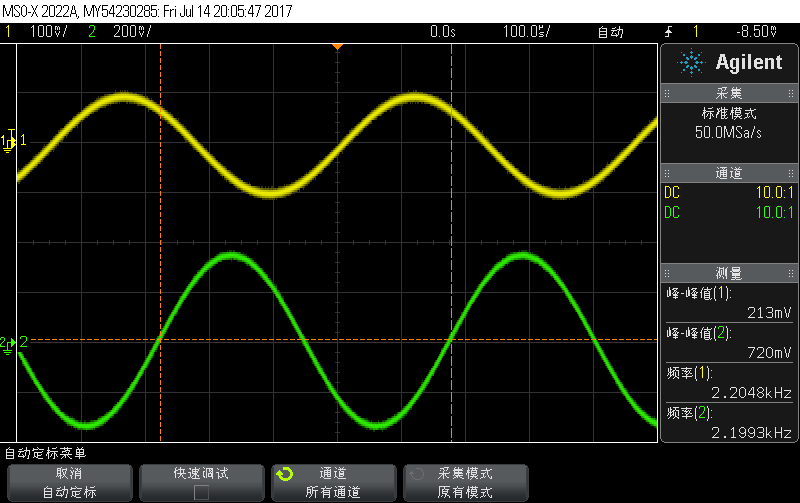
\includegraphics[width=0.6\linewidth]{imgs/scope_24.png}
	\caption{Analysis of high-pass filter}
	\label{fig-2-1}
\end{figure}

The simulation result was shown in Figure \ref{fig-2-2}.

\begin{figure}[htbp]
	\centering
	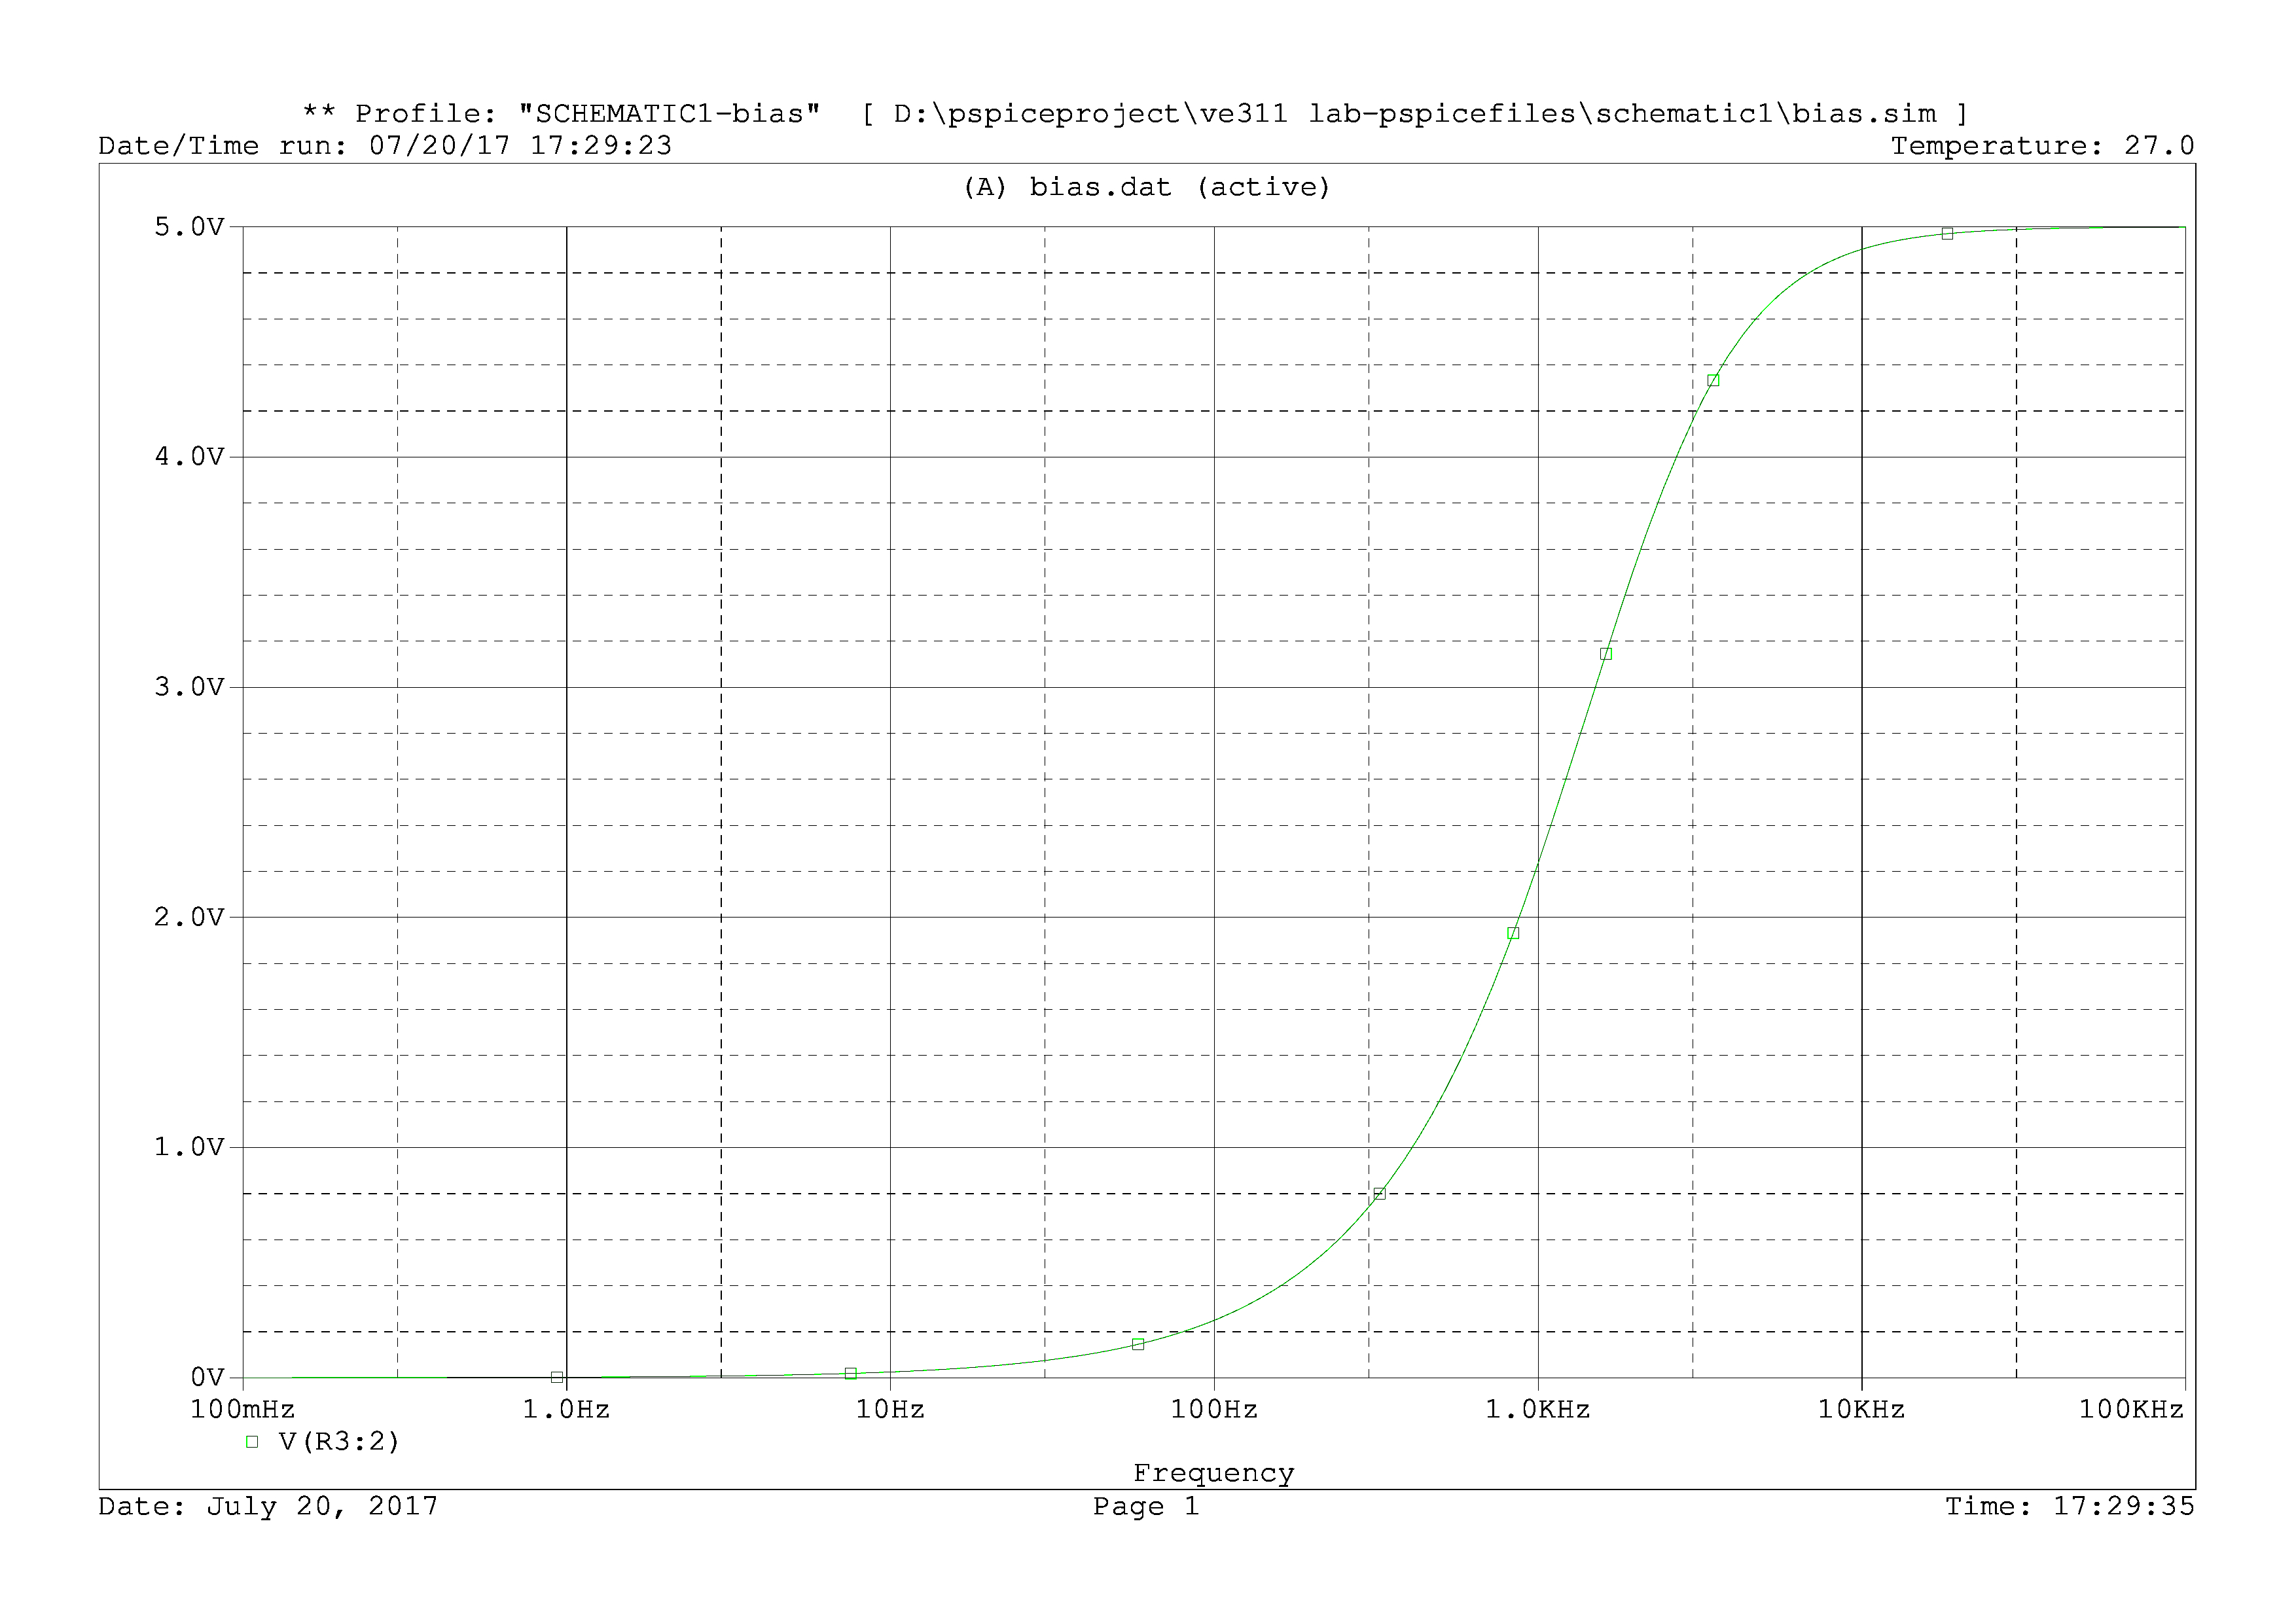
\includegraphics[width=0.6\linewidth]{imgs/high.png}
	\caption{Simulation of high-pass filter}
	\label{fig-2-2}
\end{figure}

\subsubsection{Low-pass filter}

$$f=\frac{1}{2\pi R_2C_2}$$

$C_2\approx 15.9\unit{nF}$, the result was shown in Figure \ref{fig-2-3}.

\begin{figure}[htbp]
	\centering
	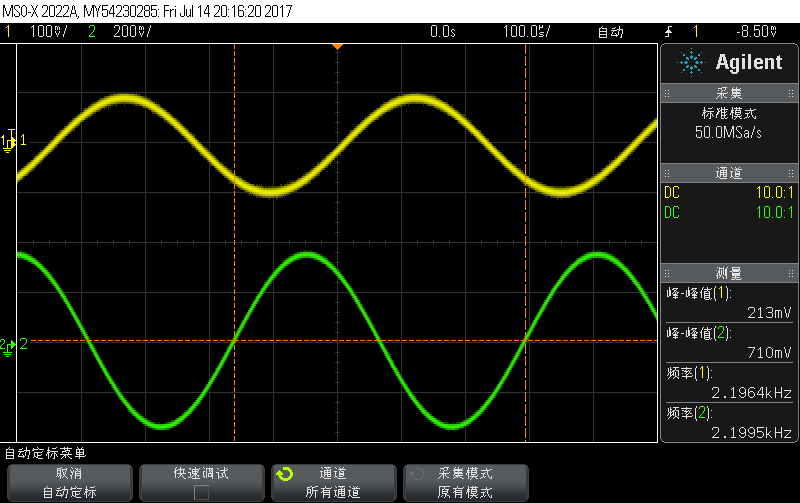
\includegraphics[width=0.6\linewidth]{imgs/scope_26.png}
	\caption{Analysis of low-pass filter}
	\label{fig-2-3}
\end{figure}

The simulation result was shown in Figure \ref{fig-2-4}.

\begin{figure}[htbp]
	\centering
	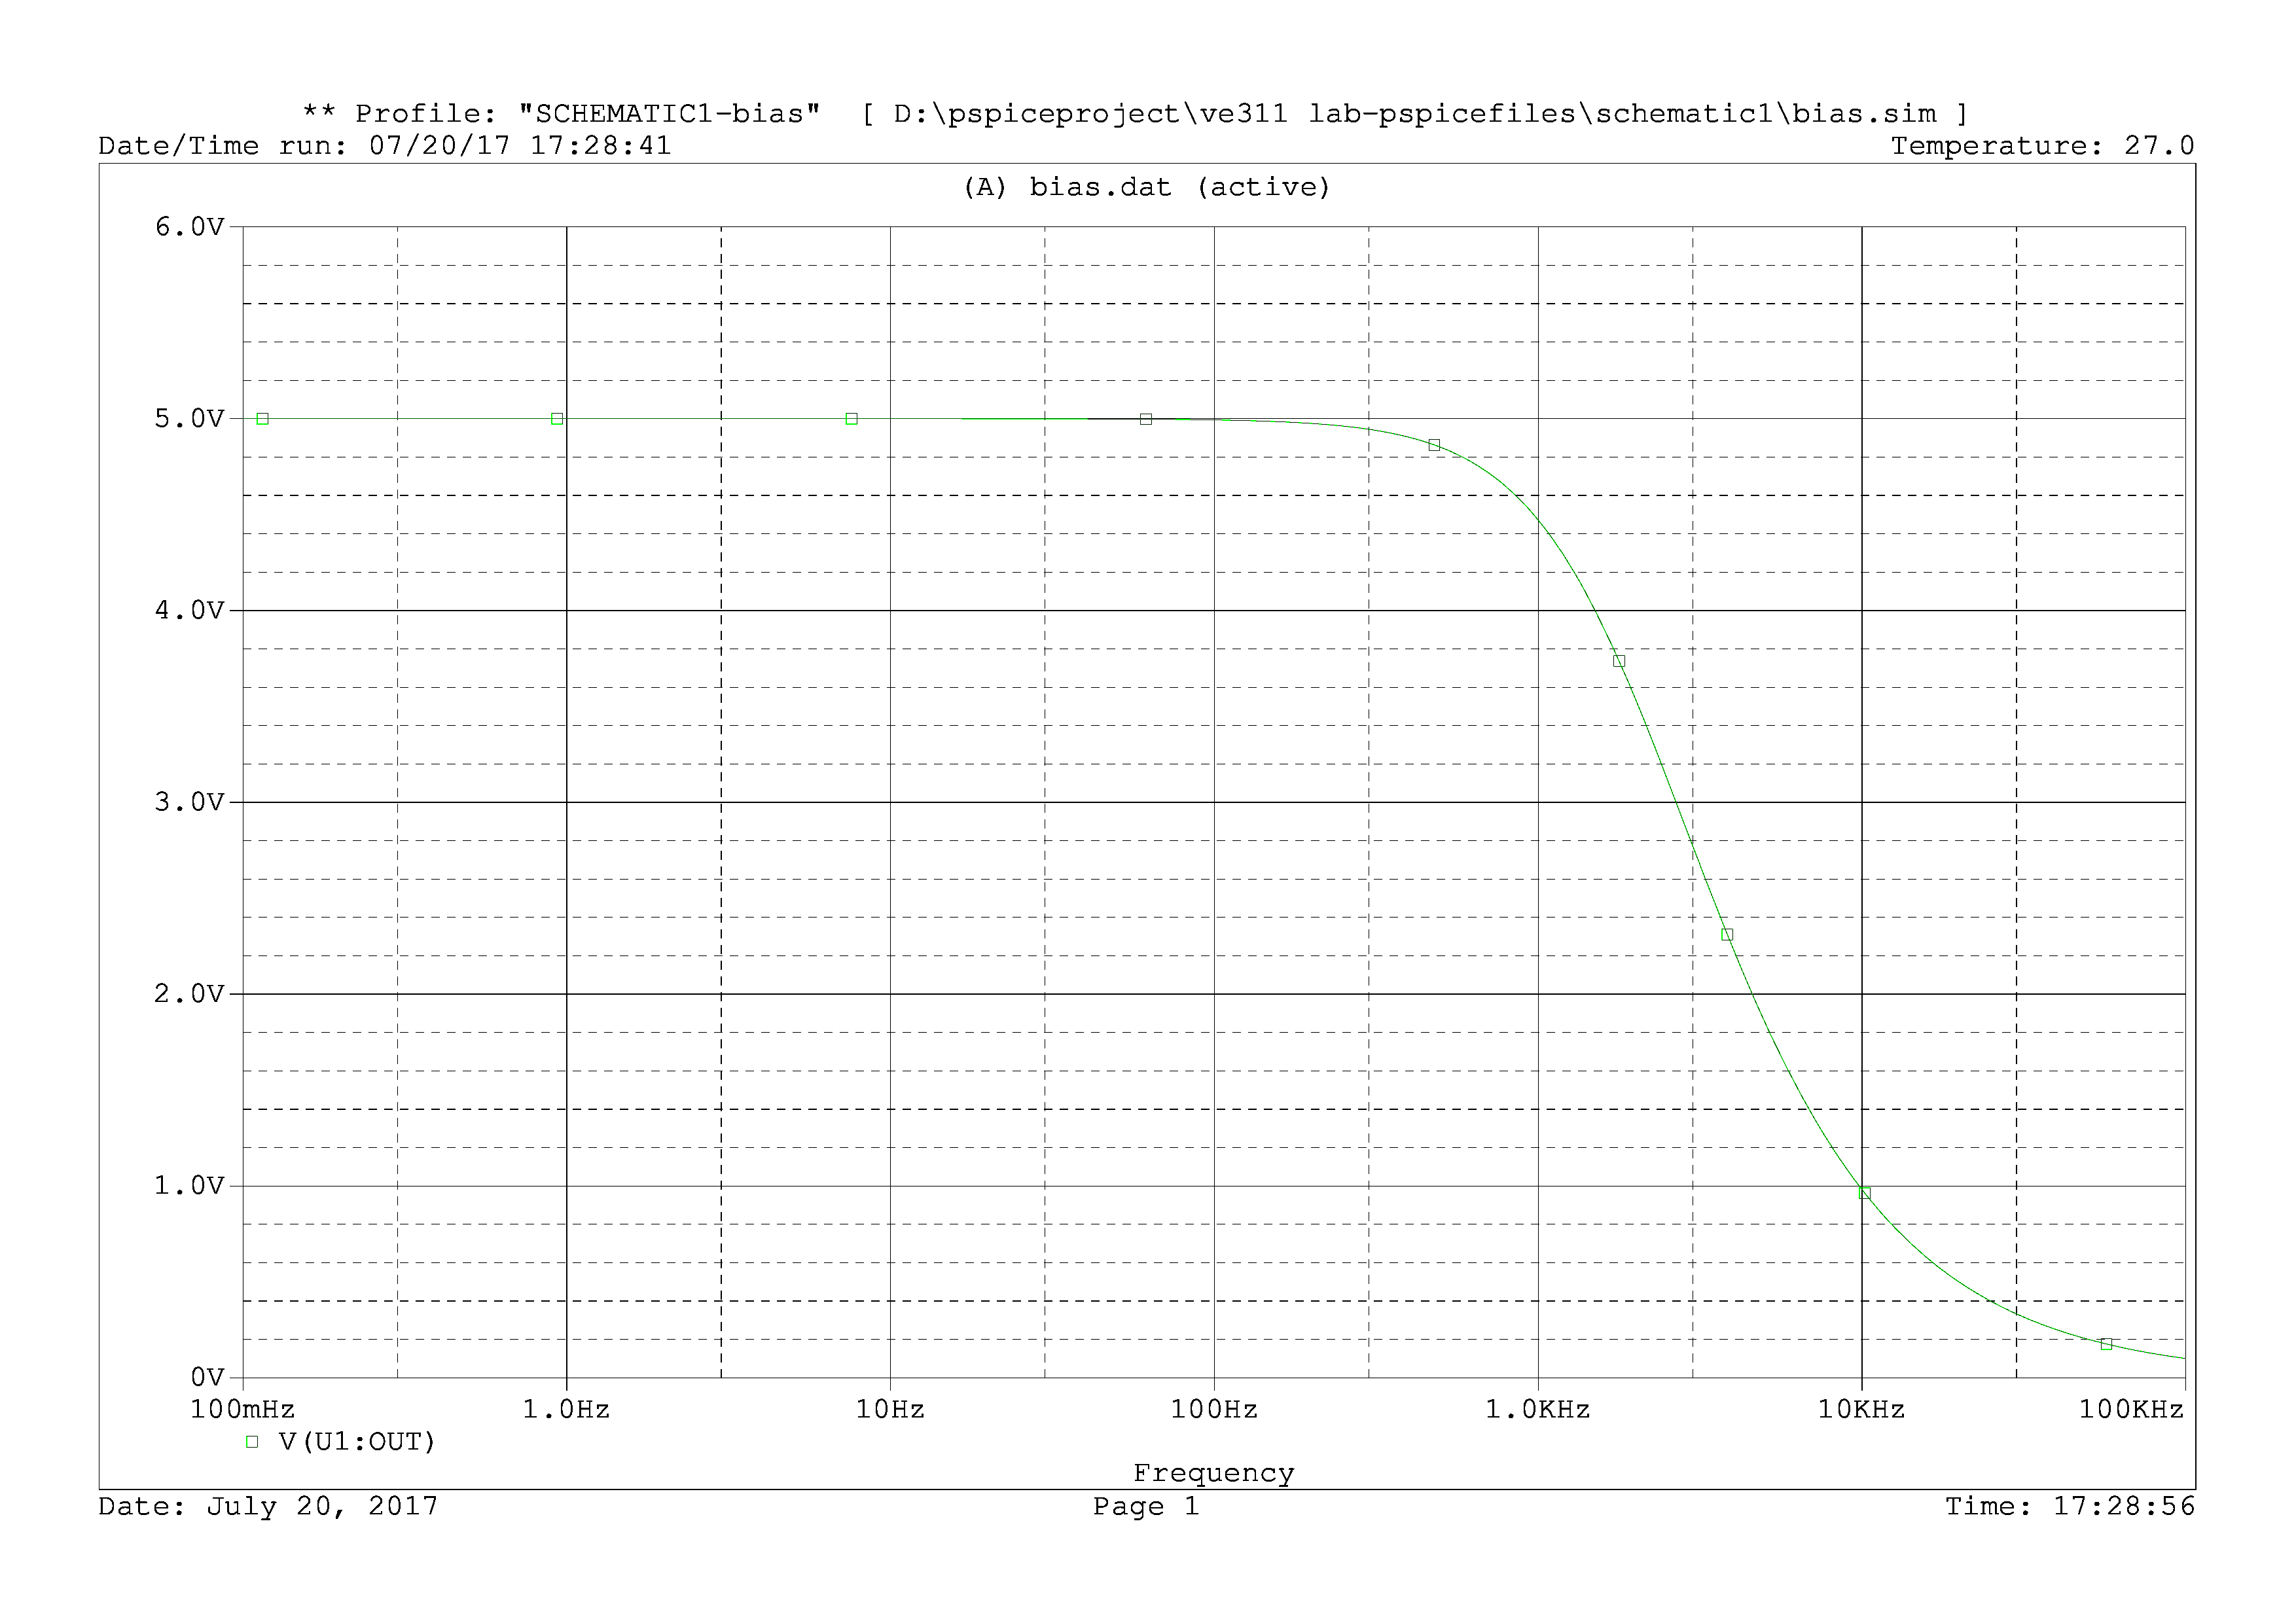
\includegraphics[width=0.6\linewidth]{imgs/low.png}
	\caption{Simulation of low-pass filter}
	\label{fig-2-4}
\end{figure}

\newpage

\section{Conclusion}

In the first part, we find the attributes of a simple amplifier.\\

In the second part, we find the relationship of cut-off frequency and resistors and capacitors. We can derive the value of capacitor of through the cut-off frequency.

We have made a mistake during the lab that we forget to connect the circuit to the ground, which leads to some strange wave shapes. Also, $\sqrt{2}$ is hard to read from the oscilloscope, some error may occurs in the process.

What we found is that the character of amplifier does not have too much connection with the change of frequency, which has some applications in practice.

\section{Reference}

\subsection{References}
\begin{enumerate}
	\item Lab5 Manual
\end{enumerate}

\end{document}
